\hypertarget{introduction}{%
\section{Introduction}\label{introduction2}}

The motivation of this thesis was twofold: firstly, to produce three-dimensional epithelia with controlled pressure, and secondly, to study the material response of the tissue to different regimes of tension. To achieve the first objective, we have developed a monolayer inflator (MOLI) device that allows us to create epithelial domes where cells can be stretched to more than 100\% of areal strain.

Epithelial tissue plays a crucial role in various physiological functions and must therefore undergo deformation over a wide range of timescales and magnitudes. Similarly, pressure levels also vary widely in different contexts \cite{torres-sanchez2021, choudhury2022a}. For instance, the luminal pressure in blastocysts doubles over the course of its development, resulting in changes in cortical tension and strain \cite{chan2019}. The MDCK dome system provides a suitable platform to investigate the interplay between cell strain, tension, and pressure. Previous studies by Latorre et al. have observed a wide range of pressure throughout the evolution of the dome, and cells have exhibited a range of deformation, including active-superelastic behavior \cite{latorre2018}. However, the control in this system is limited to the footprint of the domes, with no capability for control of pressure and tension. In this chapter, we aim to utilize the MOLI system to subject tissues to a range of strain and tension regimes.

\hypertarget{measurement-of-dome-mechanics}{%
	\section{Measurement of dome
		mechanics}\label{measurement-of-dome-mechanics}}


To measure the kinematics of the domes, we focused on the midsection, assuming symmetry of spherical caps (see Figure \ref{fig_7_1}). We measured the height ($h$) and base radius ($a$) of each dome, which allowed us to calculate the radius of curvature ($R$) using trigonometry as
\begin{equation}
	\label{eqn:radiuscurve}
	R = \frac{h^2 + a^2}{2h}.
\end{equation}
Additionally, we measured the pressure ($\Delta P$) to compute the tension ($\sigma$) using Laplace's law
\begin{equation}
	\label{eqn:laplace}
	\sigma = \frac{\Delta PR }{2} .
\end{equation}

For dome strain, we utilized the areal strain measure, which is based on the surface area, and compared the dome surface area ($A$) to the area of the footprint ($A_{0}$) by
\begin{equation}
	\label{eqn:arealstrain}
	\epsilon = \frac{A - A_{0}}{A_{0}} = \frac{\pi(h^2 + a^2) - \pi a^2}{\pi a^2} = \frac{h^2}{a^2} .
\end{equation}

However, the line scanning modality of a Zeiss Airy Scan Microscope generated hundreds of images per experiment, making manual quantification of geometrical parameters impractical. To overcome this challenge, we generated kymographs of the top section of the domes, enabling us to extract geometric information more efficiently (see previous chapter). Using these kymographs, we could measure the tension and strain of the domes with greater ease and speed. These advances have significantly enhanced our ability to explore the material properties of the epithelial tissues.


\begin{figure}
	\begin{minipage}[c]{0.7\textwidth}
		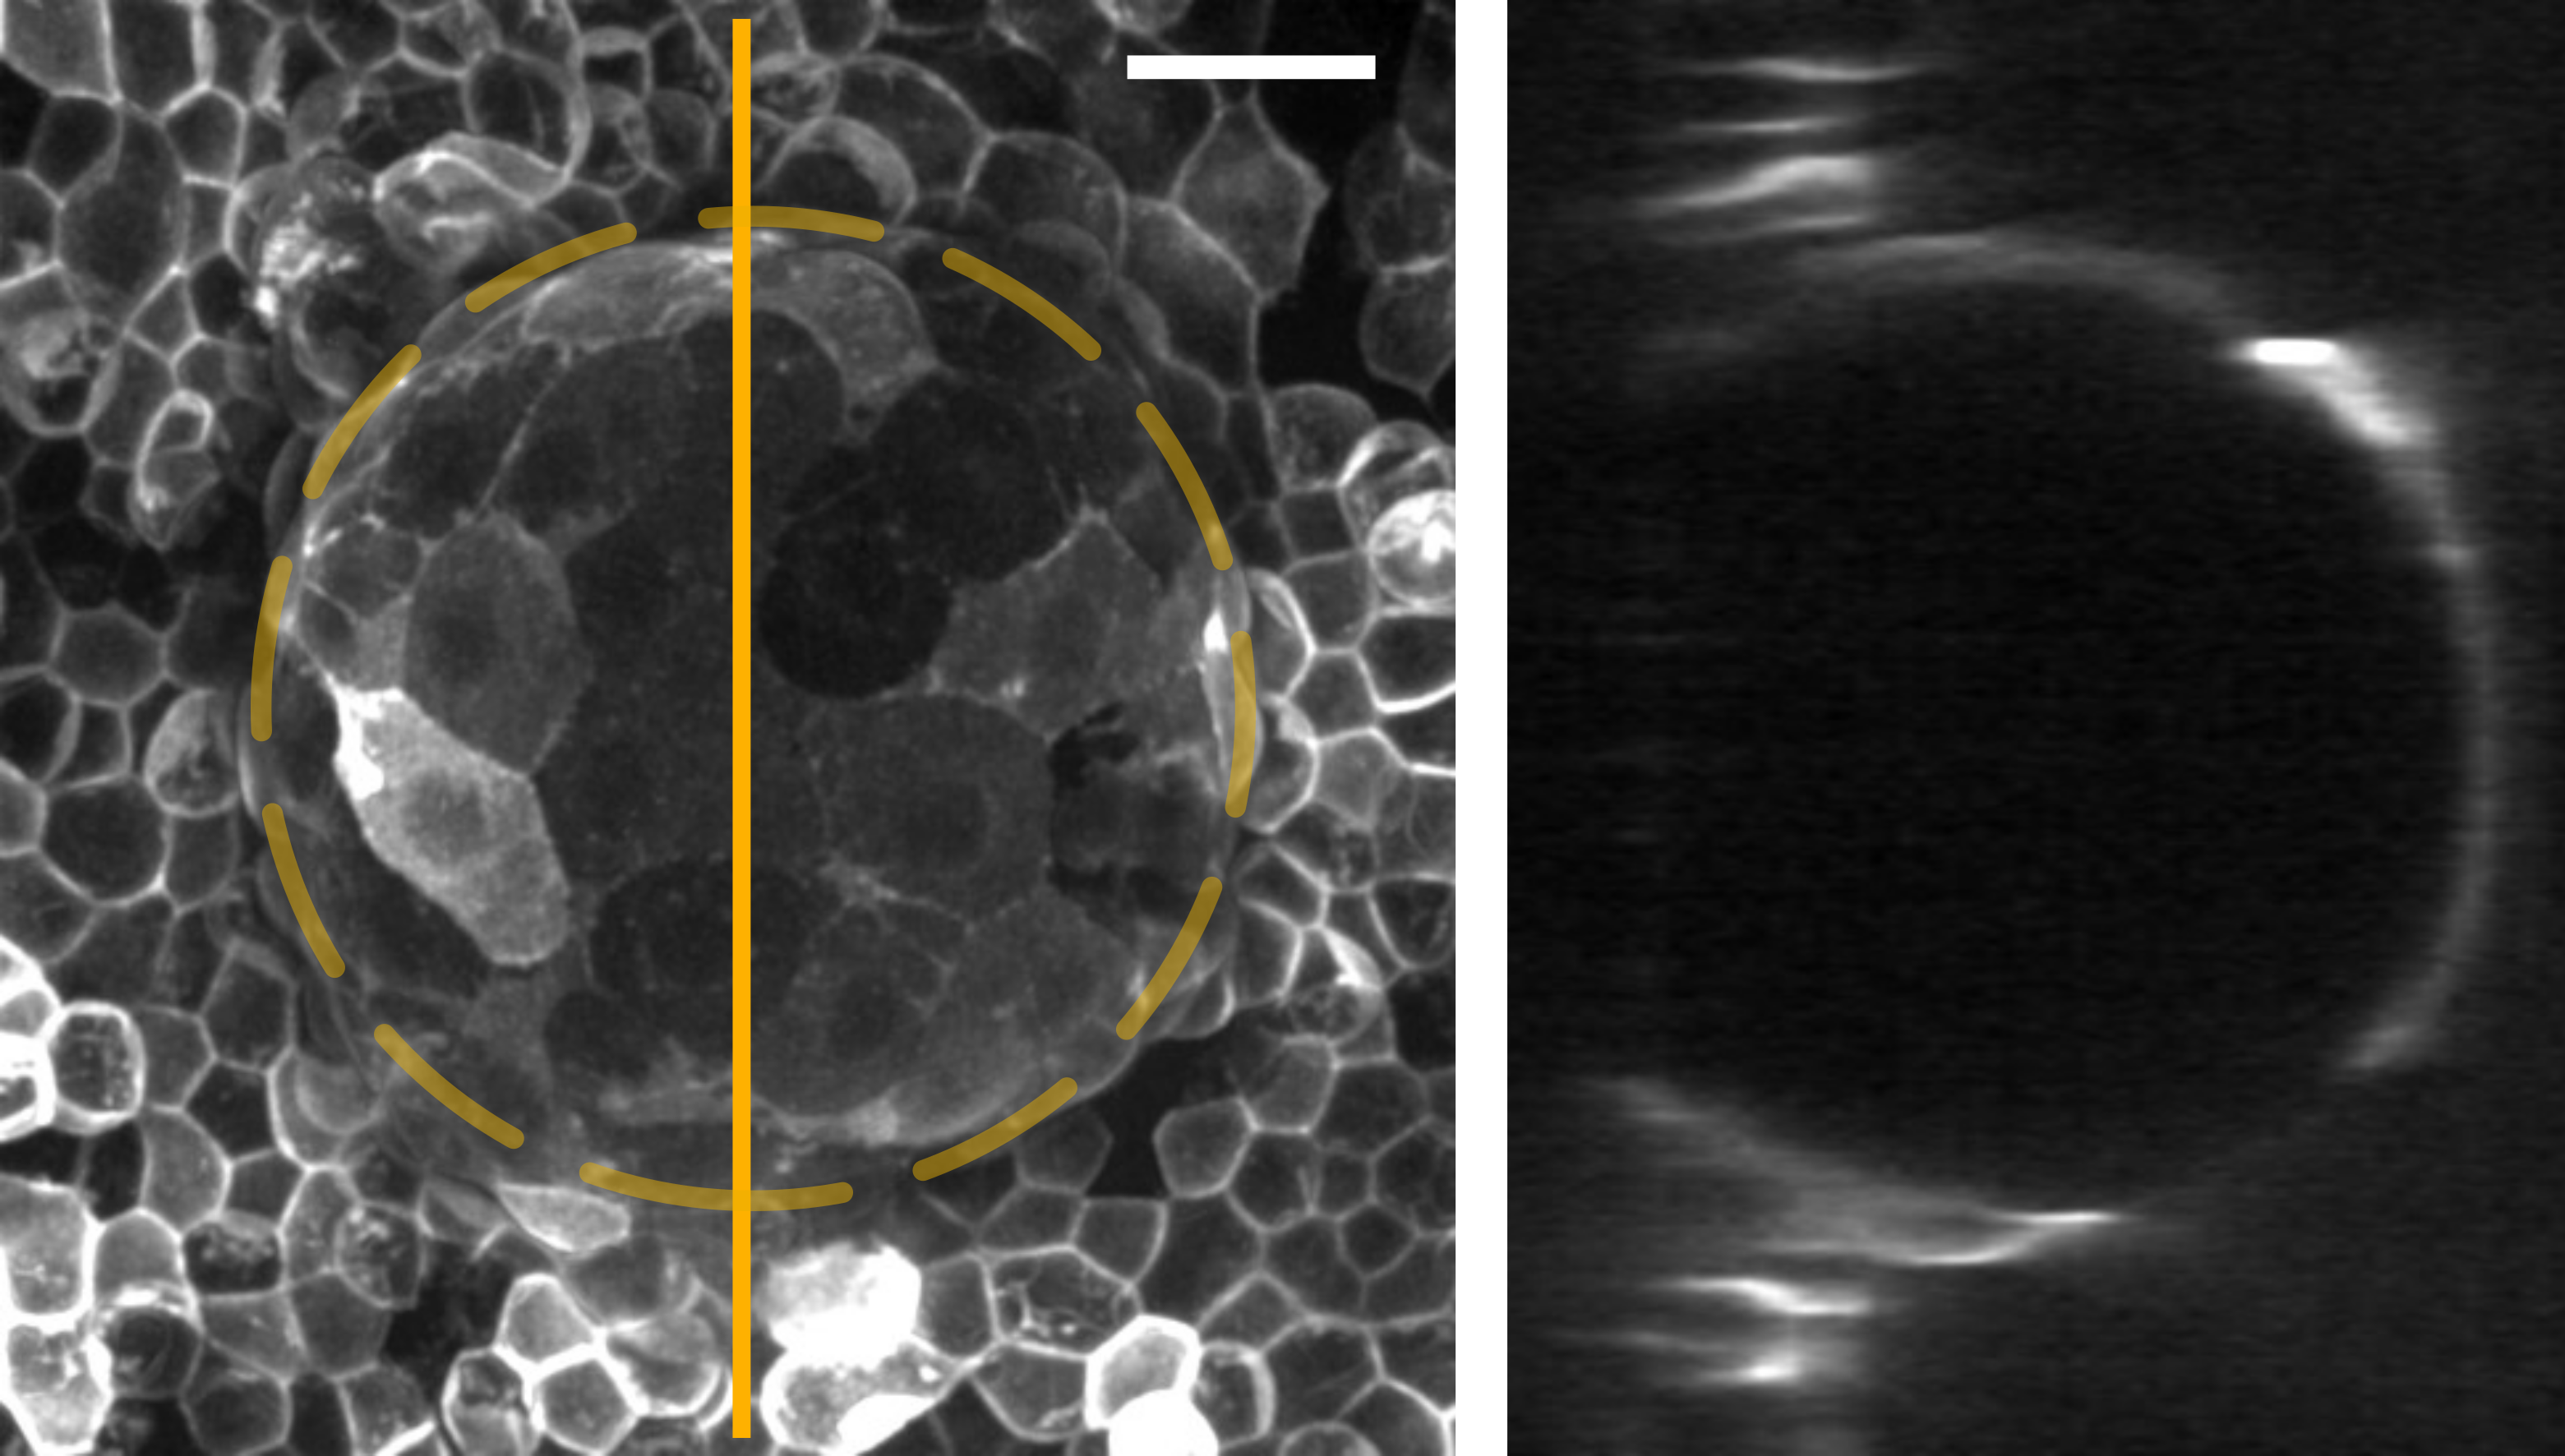
\includegraphics[width=\textwidth]{chap7_realdome.png}
	\end{minipage}\hfill
	\begin{minipage}[c]{0.27\textwidth}
		\caption{\\ \textbf{Spherical cap}:\\An example of an epithelial dome at 200 Pa, which has increased its surface area almost four times the original footprint. The spherical shape of the dome can be seen in the cross-section. Scale bar is  $20 \mu m$.
		} \label{fig_7_1}
	\end{minipage}
\end{figure}

\hypertarget{epithelial-domes-at-constant-pressure}{%
	\section{Epithelial domes at constant
		pressure}\label{epithelial-domes-at-constant-pressure}}

We systematically inflated domes at varying pressures ranging from 0-400\unit{\pascal}. However, we found that domes could not form at pressures lower than 50-100\unit{\pascal} due to adhesion forces, and delamination occurred at higher pressures. Eventually, we determined that 200 Pa allowed the domes to form without delaminating, falling within the previously reported pressure range \cite{choudhury2022,marin-llaurado2022}.

Our measurements revealed that when the domes were subjected to a constant pressure of 200\unit{\pascal}, they underwent a significant increase in areal strain during the first three to five minutes of pressure application. Following this initial increase, the areal strain reached a plateau and remained relatively constant for the next 5-10 minutes (see Figure \ref{fig_7_3} A). Notably, our findings also indicated considerable variability in dome-to-dome strain, with strains ranging from 50\% to 300\%. Nevertheless, the stabilization in strain across all the domes suggested that a steady state had been achieved by the epithelial tissue.

In analyzing the tension-strain relationship of these domes, we found that it exhibits a non-monotonic curve similar to the Nike "swish" symbol (see Figure \ref{fig_7_3} B). At low strains, the tension within the domes is exceptionally high, followed by a decline to a minimum value at an areal strain of one, where the dome adopts a hemispherical shape. The tension then increases once again, but the rate of increase is much slower than the rate at which tension decreases at lower strains. Such a material response for biaxially stretched materials is unusual.

This tension-strain relationship of the domes can be explained by the geometric constraints imposed by the dome system and force balance, as governed by Laplace's law. The tension within the dome is intrinsically dependent on its radius of curvature, and the initial high value of the radius of curvature leads to a correspondingly high tension that subsequently diminishes to a minimum upon adopting a hemispherical shape (see Figure \ref{fig_7_4}). Since the dome always maintains a spherical shape, the radius of curvature, areal strain, and tension are all interconnected. The expression of the curve can be derived by substituting areal strain ($\epsilon$) in the expression of radius of curvature ($R$) (Equation \ref{eqn:radiuscurve})
\begin{equation}
	R = \frac{h^2/a^2 + 1}{2h/a^2} = a\frac{\epsilon + 1}{\sqrt{\epsilon}}.
\end{equation}
Then, by substituting ($R$) in Laplace's law (Equation \ref{eqn:laplace}), we obtain the relation for the tension in terms of strain.
\begin{equation}
	\label{eqn:isobaric}
	\frac{\sigma}{a} = \frac{\Delta P}{4} \left( \frac{\epsilon + 1}{\sqrt{\epsilon}} \right).
\end{equation}

This relationship provides a specific link between tension and strain for a given pressure and base radius. 

Therefore, it can be inferred that when a step pressure is applied, the dome undergoes a non-steady-state with out-of-equilibrium stresses while experiencing high tension related to high radius of curvature. The dome then rapidly inflates by following the tension-strain curve dictated by equation \ref{eqn:isobaric} to achieve a steady state. In this steady state, the external pressure is balanced with tissue tension. It is evident that this Nike curve material response does not represent the quasi-static constitutive relation of the epithelial tissue. To determine the true constitutive relation, a different experimental strategy will be adopted in the following section.

\begin{figure}[t]
	\centering
	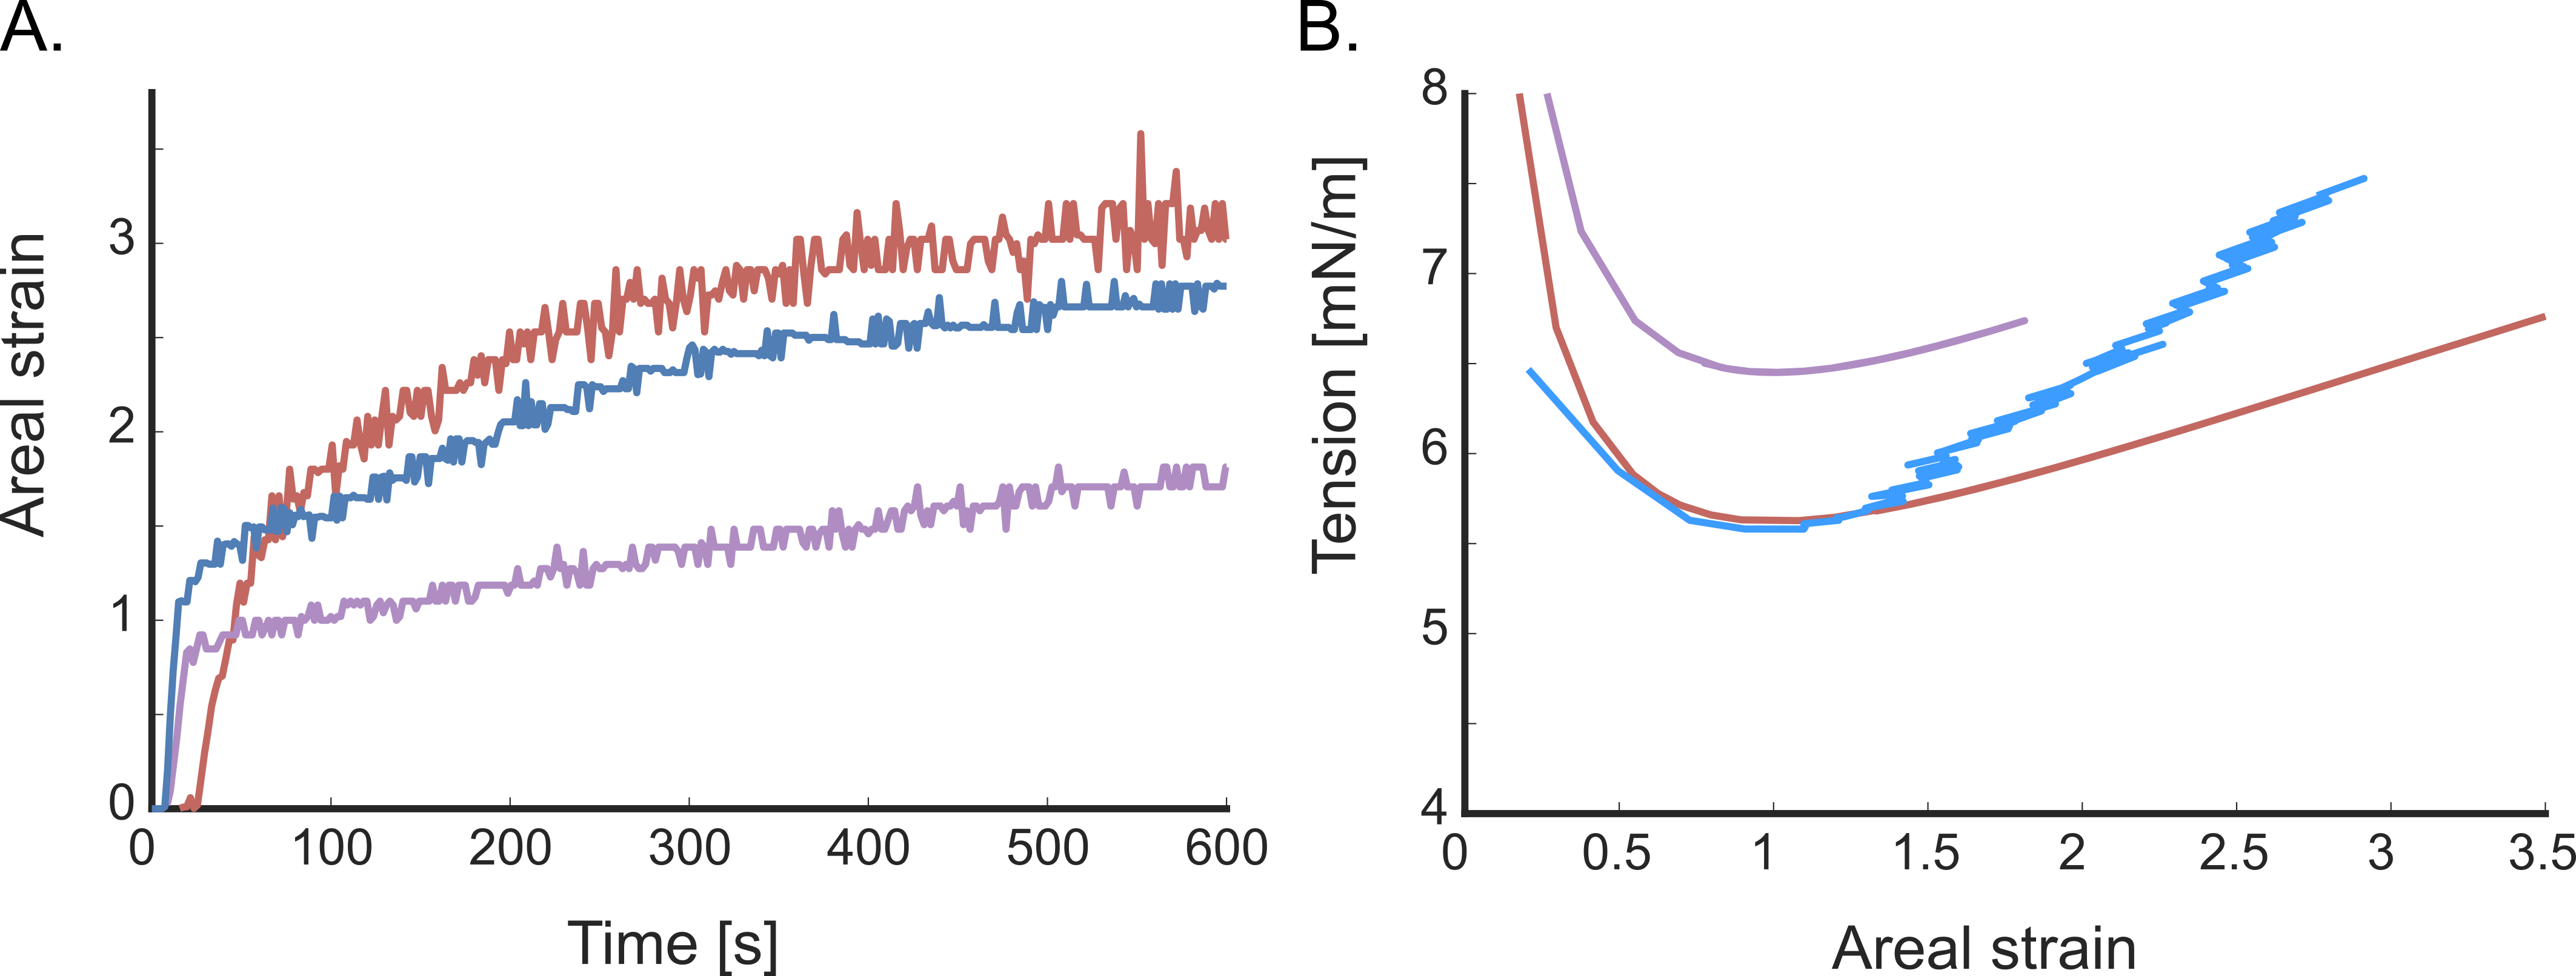
\includegraphics[width=\textwidth]{chap7_constpressure.png}
	\caption{\label{fig_7_3} \textbf{Epithelial domes at constant pressure}:Dynamic response of the representative domes at a constant pressure of 200 Pa: (A) Areal strain increases and reaches a steady state at around 5 minutes, and we can clearly see variability in the maximum strains. (B) The same domes produce a peculiar "NIKE swish" shaped tension and strain curve.
	}
\end{figure}

\begin{figure}
	\centering
	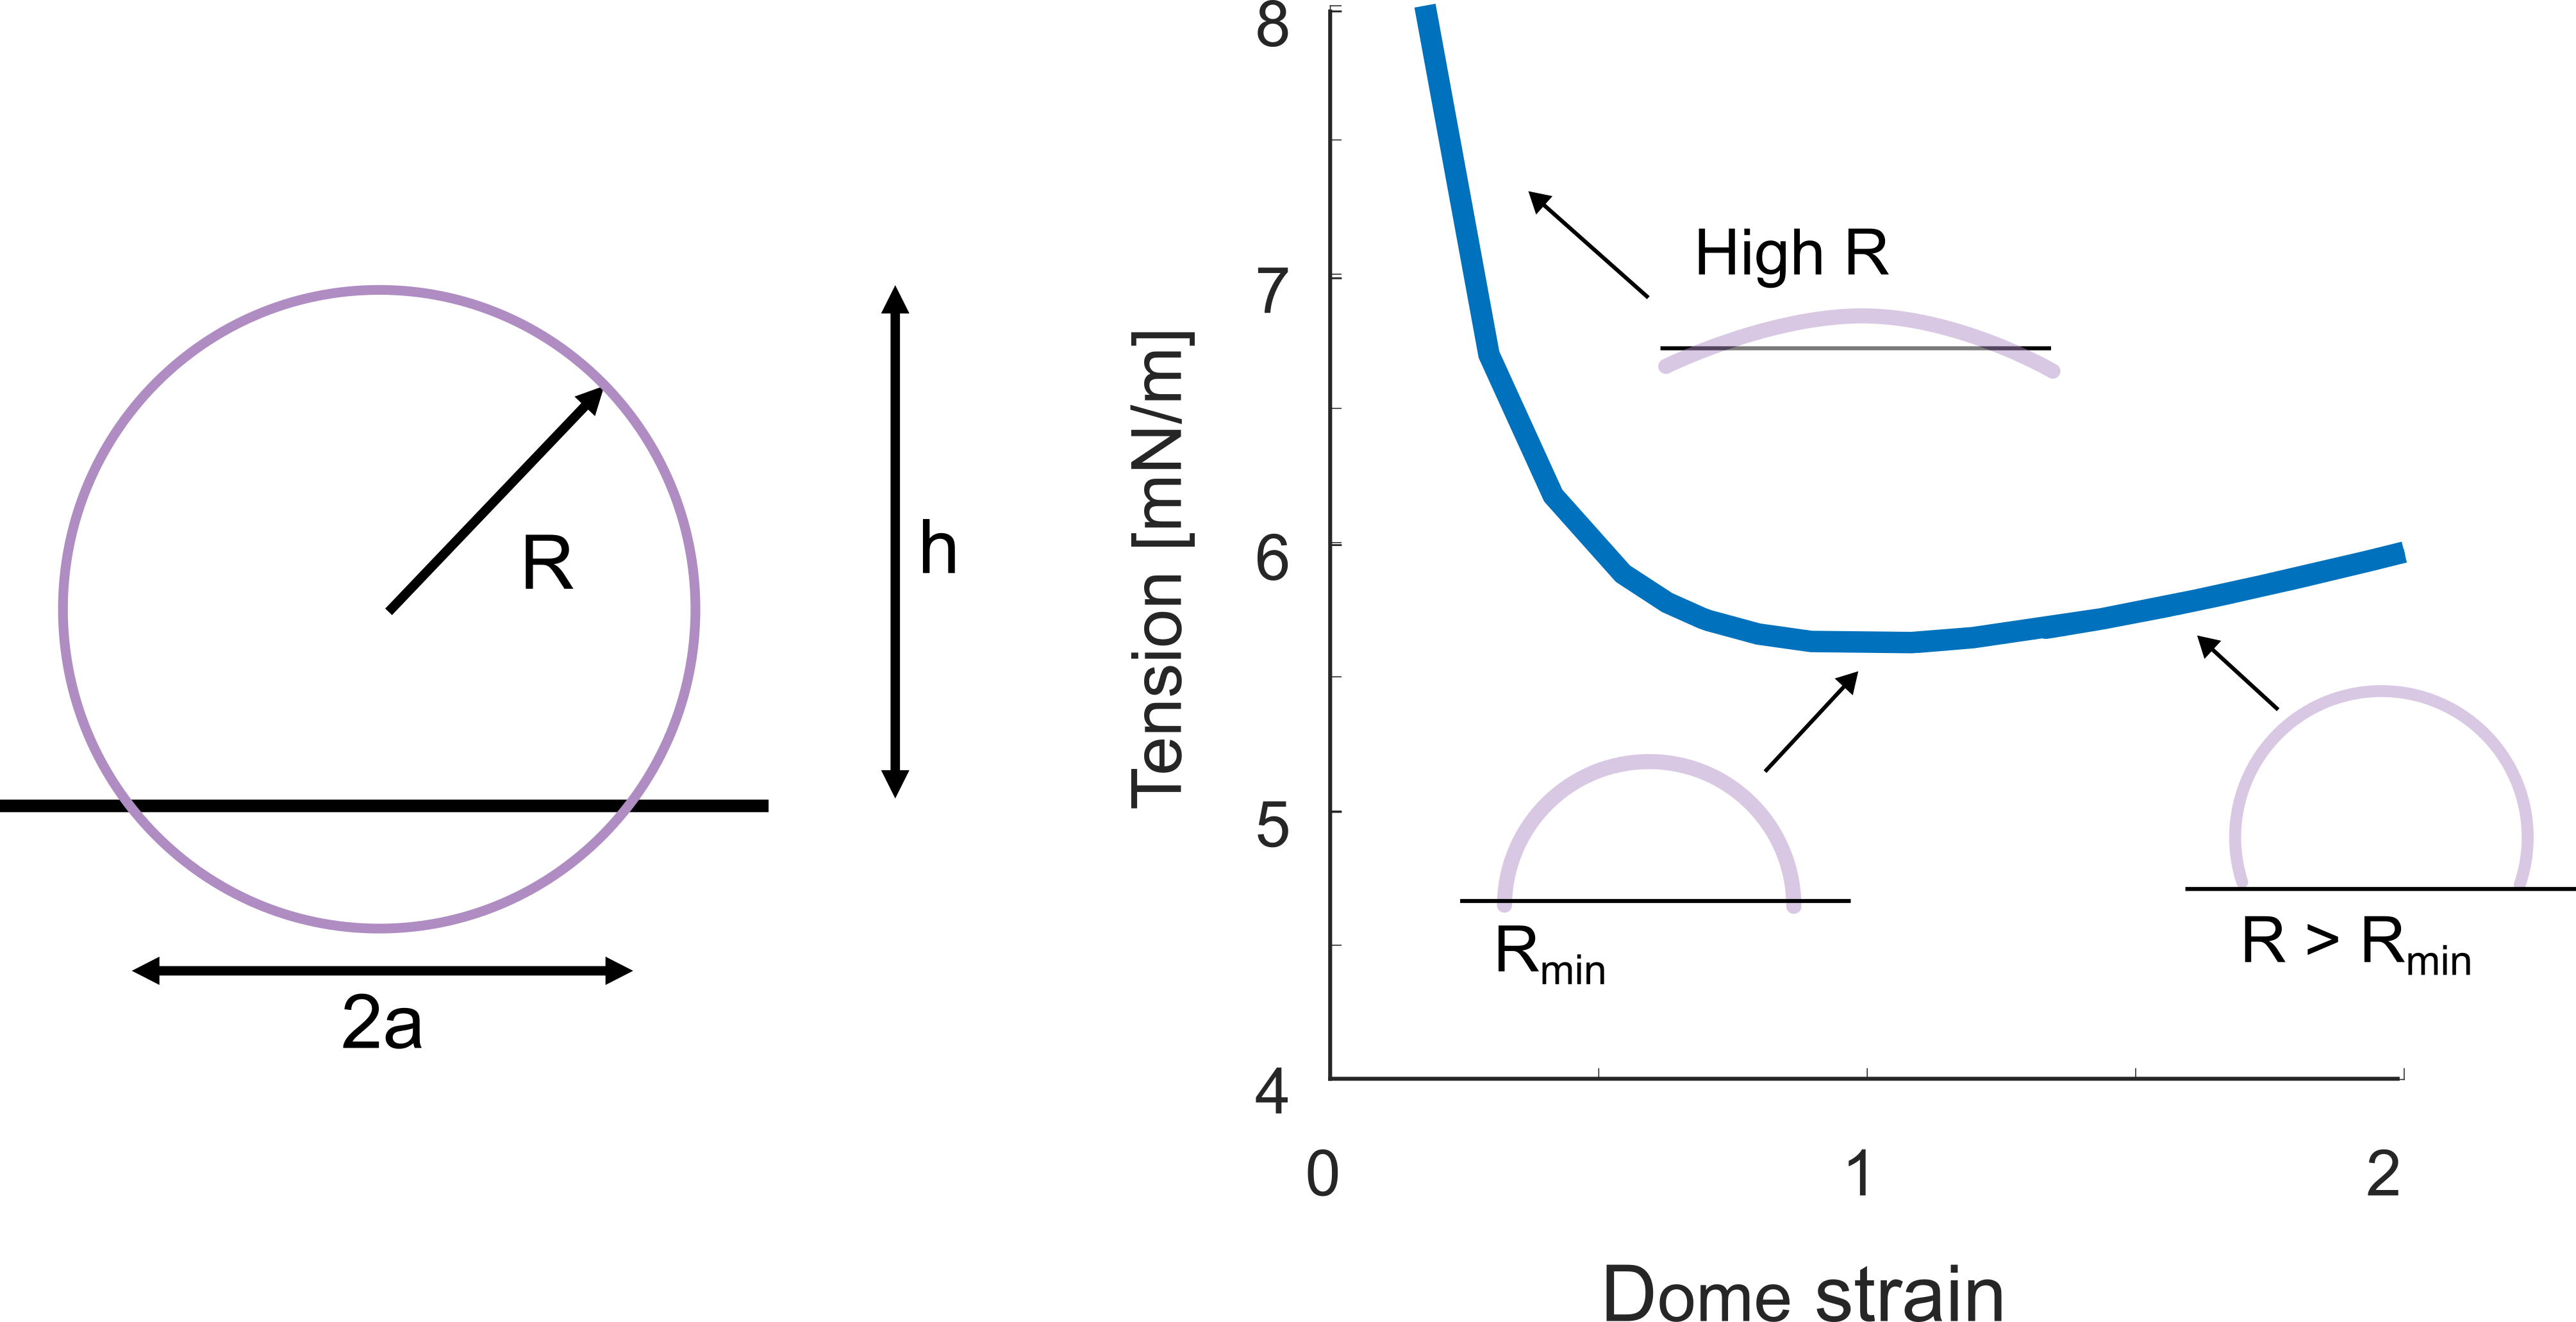
\includegraphics[width=0.8\textwidth]{chap7_radius.png}
	\caption{\label{fig_7_4} \textbf{Illustrative explanation for isobaric curve}: Tension and strain are related to each other through the geometric constraint of a spherical cap. Here, the base radius (a) is constant, so the radius of curvature is almost infinite for domes with very small strains (<0.05). As the strain increases, the radius of curvature decreases to a minimum corresponding to the base radius. Then it continues to increase again.	
	}
\end{figure}

\hypertarget{constitutive-relation-of-epithelia}{%
	\section{Constitutive relation of
		epithelia}\label{constitutive-relation-of-epithelia}}

In traditional experiments, quasi-static strain or tension is applied to determine a material's constitutive relation. However, our experiments could only control pressure. Increasing pressure slowly was not feasible for domes due to limited delamination at low pressures. To overcome this and obtain the tissue constitutive relation, we deflated a dome in steps, capturing steady-state tension and strain for different pressures. The locus of these steady states provides the constitutive relation.

We applied a pressure of 200 Pa for 5 minutes, allowing the dome to reach a steady state. We then reduced the pressure in increments of 20 Pa, permitting the dome to reach steady state at each step (see Fig. \ref{fig_7_5}). This process continued until the dome was completely deflated. Consequently, we captured the material response of the tissue at various pressures as the dome transitioned through different tension-strain states. It appeared to move between different Nike curves corresponding to pressure. By mapping all steady-state tension-strains of domes at different pressures, we determined a constitutive relation for the tissue.

The resulting constitutive relation showed an initial increase in tension with strain for lower strains. For larger strains, the tension plateaued, consistent with earlier studies on MDCK domes (see Fig. \ref{fig_7_5} B). It is important to note the significant variability in dome-to-dome tension, with recorded tensions around 4.5 mN/m aligning with the same order of magnitude as those in previous studies (Latorre2018, Marin-Llaurado2022).

To summarize, our experiments demonstrate that the tissue reaches a steady state under a specific static pressure, which enables us to determine its constitutive relation through deflation. In the next section, we will explore the dynamic material response of the tissue.

\begin{figure}
	\centering
	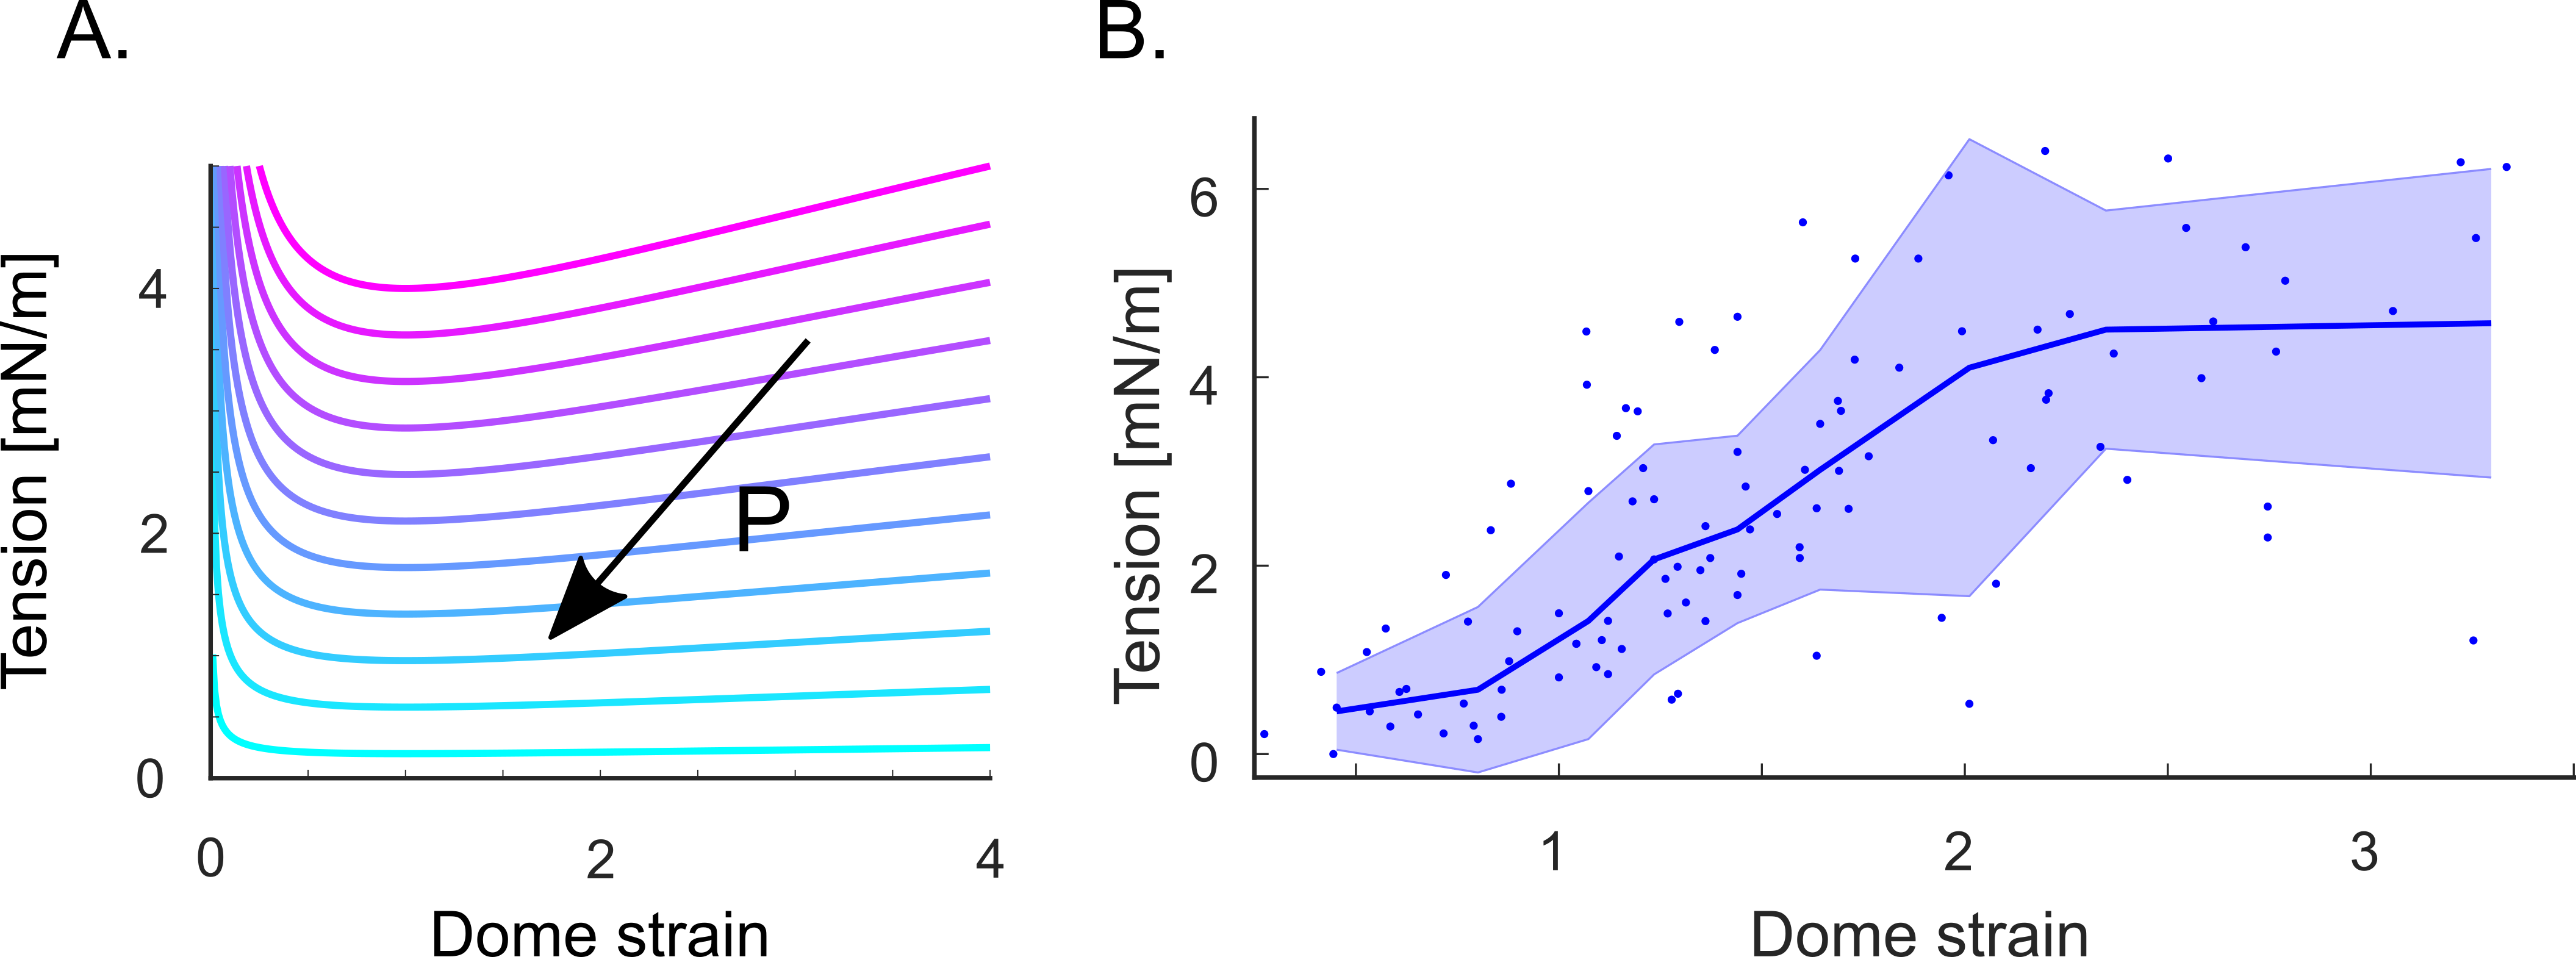
\includegraphics[width=\textwidth]{chap7_constitutivelaw.png}
	\caption{\label{fig_7_5} \textbf{Constitutive Relation of Epithelia}: (A) We will set up experiments to probe the steady state at different pressures. We will start from the highest pressure, move along the isobaric line and achieve a steady state, and then move down to the next curve, and so on.	(B) The constitutive relation between dome strain and tissue tension was experimentally obtained (n=12). The line and shaded area represent the median and standard deviation, respectively, by binning 13 points in each bin.
	}
\end{figure}


\hypertarget{dynamics-of-the-epithelia-domes}{%
	\section{Dynamics of the epithelia
		domes}\label{dynamics-of-the-epithelia-domes}}

In this section, we investigated the dynamic material response of the domes by conducting cyclic stretching experiments. We subjected the domes to a triangular wave of pressure with a magnitude of 200 Pa at three distinct timescales, as depicted in Figure \ref{fig_7_6}. The selected timescales of 20s, 266s, and 2000s were based on existing literature on tissue remodeling, particularly the work of Khalilgharibi et al. (2019) and Casares et al. (2015) \cite{khalilgharibi2019, casares2015}. These studies demonstrated that stress relaxation experiments in tissues occur from tens of seconds to minute timescales due to F-actin remodeling and myosin-driven contractility. Additionally, in some cases, even faster deformation at timescales of a few seconds has been shown to impact cell remodeling \cite{andreu2021a}. In our device, the fastest cycle that could be probed was limited to 20s because of the microscope's imaging speed.

\begin{center}
	\begin{table}[h!]
		\label{tab:hysteresis}
		\begin{tabular}{c c c c}
			& Fast & Moderate & Slow \\ 
			Time period (s) & 20   & 266      & 2000 \\ 
			Rates (Pa/s)    & 20   & 1.5      & 0.2  \\ 
		\end{tabular}
	\end{table}
\end{center}

For the fastest cycles, we observed that the maximum strain achieved by the domes in each cycle increased until they reached a steady state oscillation around 600 seconds. The experiment was conducted over 1200 seconds, equivalent to 60 cycles, during which we observed a cumulative buildup of strain over time. In the loading phase, the domes underwent stretching, while during the unloading phase, they experienced unstretching but failed to revert to zero strain after the initial cycles. In the concluding cycles, we noted that the dome oscillated between two distinct states of strain, resembling a limit cycle.

A similar response was observed for the moderate cycles, where the domes were stretched for five cycles of 266s each. The strain accumulated in the first cycle, with strains reaching higher values than those observed in the fast case. Moreover, after a few cycles, the dome appeared to reach a stable limit cycle.

For the slowest cycles, spanning a duration of 4000 seconds, we observed that the domes did not form at lower pressures. As previously discussed, the domes remained attached until a pressure of 100-150Pa was attained, beyond which they underwent rapid inflation, leading to high strains of 200-350\%. However, in cyclic stretching, we noted that strain accumulation did not occur, and there was no variation in the maximum strains attained during both cycles.

Through these experiments, we clearly observed the rate-dependent response of the domes. At faster rates, domes accumulated strains, while at slower rates, they could undergo large, reversible deformations. This behavior resembles viscoelastic properties. In the next section, we will further explore this viscoelastic behavior to better understand the tissue's characteristics.

\begin{figure}[]
	\centering
	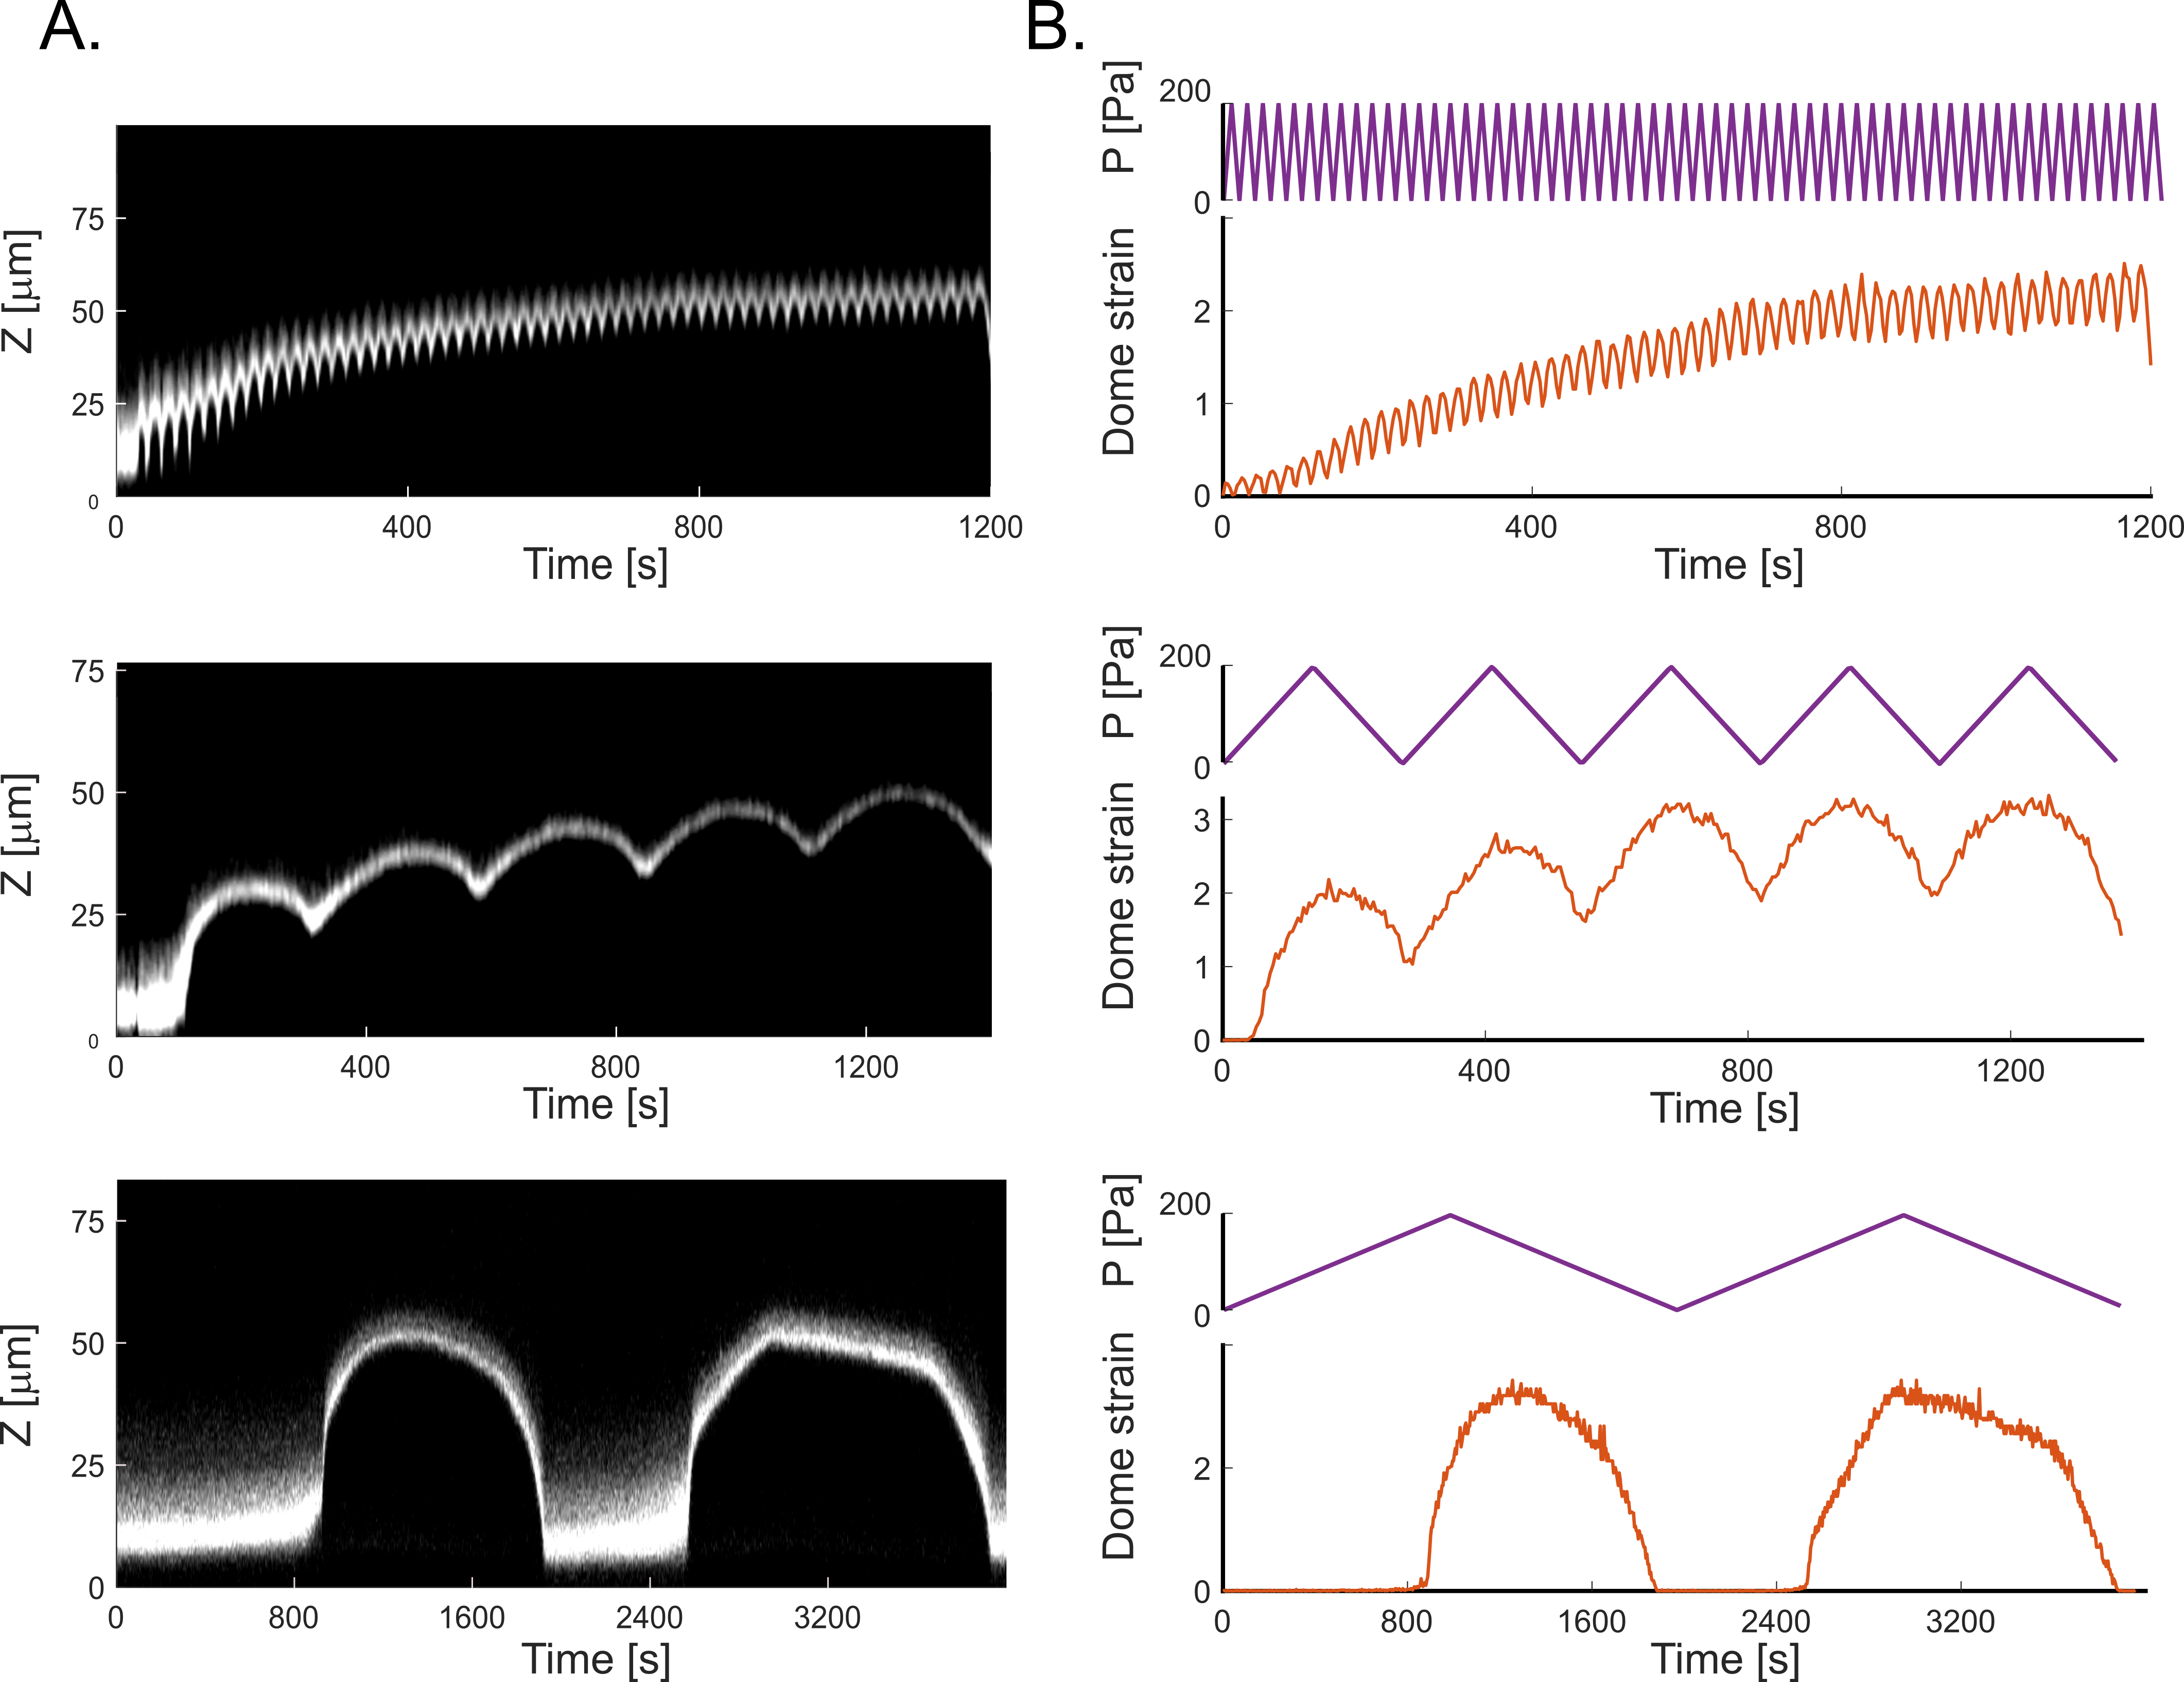
\includegraphics[width=\textwidth]{chap7_dynamic.png}
	\caption{\label{fig_7_6} \textbf{Dynamic response of Epithelia:} (A) The XZ plane images and kymographs of domes subjected to cyclic pressure between 0 to 200 Pa with rates of 20, 1.5, and 0.2 Pa/s The kymographs generated along the midsection of the domes indicated by yellow dotted lines. These indicate the evolution of height of the domes with respect to time. (B) The strain response of domes to cyclic pressure with different rates. Magenta represents pressure and red represents strain with respect to time. For A, B, n= 7 domes for 20 Pa/s, n = 8 for 1.5 Pa/s, and n = 7 for 0.2 Pa/s. 
	}
\end{figure}

\hypertarget{active-gel-tissue-model}{%
	\section{Active gel tissue model}\label{active-gel-tissue-model}}

The existing literature on epithelial mechanics emphasizes the crucial role of actin cortex viscoelasticity in sustaining deformations over timescales ranging from seconds to minutes \cite{kelkar2020,clement2017,khalilgharibi2019}. Adam Ouzeri and Marino Arroyo developed a computational model that bridges active gel models of the actomyosin cortex with 3D vertex models at tissue scales \cite{ouzeri2023}. Our collaboration necessitated close coordination, with Adam Ouzeri developing the model and me conducting experiments, facilitating the effective integration of the model with experimental data.

The model simplifies the complex cortex, comprising the actin filament network, hundreds of actin-binding proteins, and myosin motors, into a thin layer of contractile gel. This layer possesses a thickness denoted as cortical thickness ($\rho$).

The crosslinked actin filament network exhibits the behavior of an elastic network of semi-flexible filaments. Material properties are represented by Lamé parameters ($\mu$). Consequently, upon deformation, it can store elastic energy, although only at shorter timescales. At longer timescales, in response to stretching, the network dynamically reorganizes itself, releasing the stored elastic energy by relaxing stresses. This takes place through assembly/disassembly of the filaments or binding/unbinding of the crosslinkers. The dissipation of stresses is represented by a viscosity coefficient ($\eta$).

However, the active component of the active gel model arises from myosin motor activity, generating contractile active tension in the network. This active tension ($\gamma$) is hypothesized to be directly proportional to cortical thickness.

\begin{equation}
	\gamma(\rho) = \xi \rho.
\end{equation}

Several assumptions underlie this model. First, the cell volume is assumed to be conserved throughout the deformations. Second, cells cannot stretch indefinitely due to physiological constraints, such as reorganization of intermediate filaments, cell crowding, or compression of the nucleus. To limit strains, a strain stiffening mechanism is introduced, activated beyond really high strains.

Regarding the actin network, it is assumed to be isotropic, whereas in reality, it also be polar or nematic. Another assumption posits that the cortex undergoes constant turnover, maintaining a steady-state cortical thickness.

In the model, each cell is represented by an active gel surface that accounts for the cortex's physical attributes. A tissue is constructed from an assembly of these active gel surfaces, as depicted in Figure \ref{fig_7_2}. The system's dynamics are formulated through a balance of diverse potentials, representing free energy, dissipation, active internal, and external forces.

Due to this formulation, the system exhibits the behavior of an active hyperelastic material at shorter timescales, while at longer timescales, it behaves like an active viscoelastic material. This behavior can be explained through three timescales emerging from the theoretical framework: turnover timescale $t_{to} = 1/k_d$, viscoelastic timescale $t_{ve} = \eta/\lambda$, and viscoactive timescale $t_{va} = \eta/\xi$. The turnover timescale is driven by the cortex's polymerization rates. The viscoelastic timescale is a ratio of the viscous remodeling coefficient to the Lamé parameters, representing elasticity. Lastly, the viscoactive timescale is the ratio of the viscous remodeling coefficient to the coefficient of active tension.

Using this model, we generated a virtual representation of the cell monolayer, including specific regions devoid of basal attachment to the substrate, which could be inflated into domes under pressure, similar to the experimental setup. These regions will be referred to as "digital domes" in subsequent discussions (see Figure \ref{fig_7_2}). By employing this model and comparing the results with the experimental data, we could effectively understand and investigate the biomechanical properties of the epithelial tissues, specifically the contribution of the actin cortex's viscoelasticity.

\begin{figure}[]
	\centering
	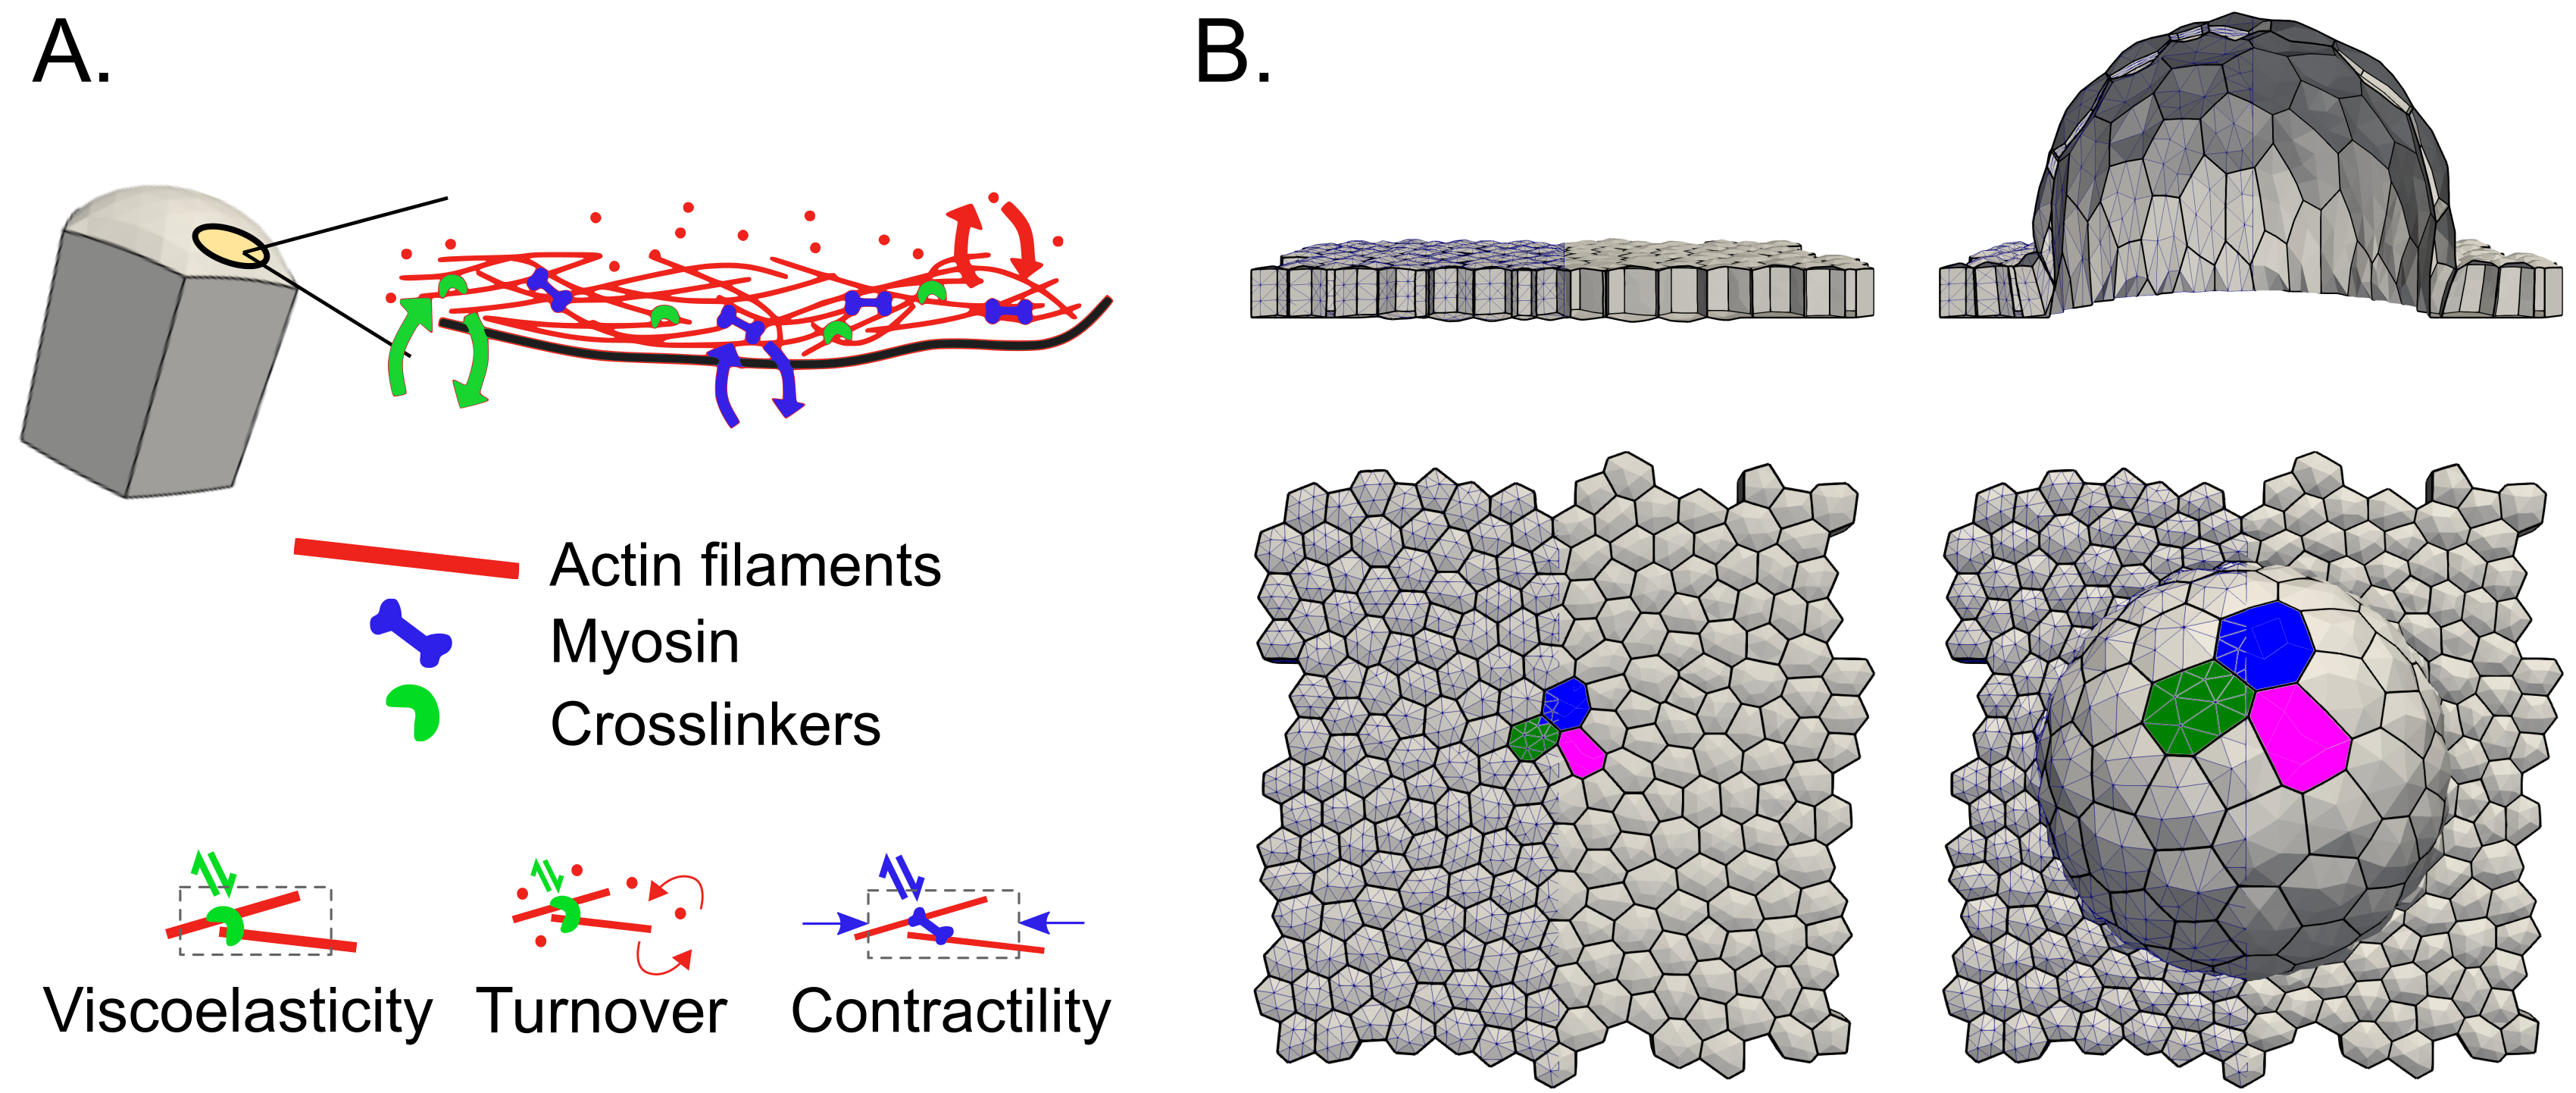
\includegraphics[width=\textwidth]{chap7_digitaldome.png}
	\caption{\label{fig_7_2} \textbf{Active gel tissue model}: (A) The cell is modeled as an active gel of cortex, which mainly comprises three aspects: viscoelasticity of the network, turnover dynamics, and active contractility. (B) These cells can be assembled into a tissue that can be used to perform in-silico experiments. An example of this is the digital dome being inflated, highlighting individual cells increasing their area.}
\end{figure}

\hypertarget{active-viscoelasticity-of-the-epithelia}{%
	\section{Active viscoelasticity of the
		epithelia}\label{active-viscoelasticity-of-the-epithelia}}
	
	
	
To investigate the active viscoelasticity of epithelia, we conducted simulations that mirrored the experimental conditions. Under constant pressure, the digital domes reached a steady state while undergoing a reduction in cortical thickness as the cells stretched. Consistent with our earlier experimental observations, once the tissue tension was balanced by the applied pressure, the strain reached a stable point (see Figure  \ref{fig_7_7} ).

To derive the constitutive relation within the computational framework, we subjected the digital dome to varying levels of pressure, generating tension-strain curves and steady-state points. The material response of the domes followed the geometric constraint observed in experiments, resulting in a non-monotonous tension-strain curve.

In addition, a quasi-static inflation of the digital dome was performed to assess the model's robustness. The quasi-statically obtained constitutive relation showed consistency with the locus of steady-state tension-strain points under different constant pressure conditions, as shown in Figure \ref{fig_7_7} B. The resulting constitutive curve also demonstrated characteristics similar to those obtained experimentally, including re-stiffening at significant strains attributed to a barrier mechanism. (see Figure \ref{fig_7_7} A).

To interpret these experimental results in the context of the model, we introduced the concept of the resting area, which could aid us in understanding the active viscoelasticity. The mathematical framework used in the model describes how the cortical surface changes its shape when deformed. This framework maps the initial shape (known as the reference configuration) to its current shape (known as the deformed configuration), with a corresponding metric tensor\footnote{The metric tensor is used to measure distances and angles within the material. When a material is deformed, the distances and angles within the material change, and the metric tensor reflects these changes.} for each configuration. To capture remodeling of the cortex, a second reference configuration is added with a dynamic metric tensor, where the cortex has relaxed. We could refer to this as the resting frame.

In terms of cell area, the current area is the actual area represented by the deformed configuration. However, the cell could have a resting area different from the actual area, represented by the second reference configuration due to network relaxation.

\begin{equation}
	A_{rest} = \int_{\Gamma_0} \sqrt{|\mathbf{G}|}dS_0, \text{ and } A_{actual} = \int_{\Gamma}dS.
\end{equation}

When the tissue is perturbed from this state, the actual area can change faster than the resting area due to the viscoelastic behavior of the tissue. The cell dissipates elastic stresses at viscoelastic timescales through remodeling, eventually reaching a steady state. This effect of timescales is particularly evident in cyclic stretching experiments. When the cells are probed faster than viscoelastic timescales, they accumulate strains due to an inability to dissipate the elastic stress. In contrast, when stretching is slower, elastic stresses are dissipated with increasing area.

We observed that, for the slowest condition, the resting area in the digital dome almost overlapped with the actual area. This is because the pressure is changing very slowly at a rate of 0.2 Pa/s, allowing the cells sufficient time to remodel and dissipate elastic stresses. Viscoelastic and turnover timescales in simulations are around 10-30s, which means that over a period of 2000s, the dome stretches considerably and returns to original flat state.

However, when pressure is applied rapidly in cycles of 20 seconds, strains accumulate due to insufficient time for cells to dissipate stored elastic energy. The simulations show that the resting area marginally changes relative to the actual area. Notably, creep experiments, where tissue is stretched at constant tension, demonstrate strain accumulation at the visco-active timescale, where both contractility and viscosity play a role.

Interestingly, the simulations indicate that due to active viscoelasticity, there would be a lag between the peak of pressure and the peak of strain. This lag is clearly reflected in the comparison of resting area and actual area, where the delay decreases with increasing pressure rates. The slowest pressure rate results in the least amount of delay, while the fastest pressure rate results in the most delay. Although we can only experimentally observe this at moderate rates. The experimental data from faster cycles is too noisy to observe the lag.

To sum up, the digital dome model explains the material response of epithelial tissue depending on the rate at which pressure is applied. Slower rates allow for cell remodeling and dissipation of elastic stresses, while faster rates result in strain accumulation due to insufficient time for dissipation. This active viscoelastic behavior is the outcome of cortical remodeling.

\begin{figure}[t]
	\centering
	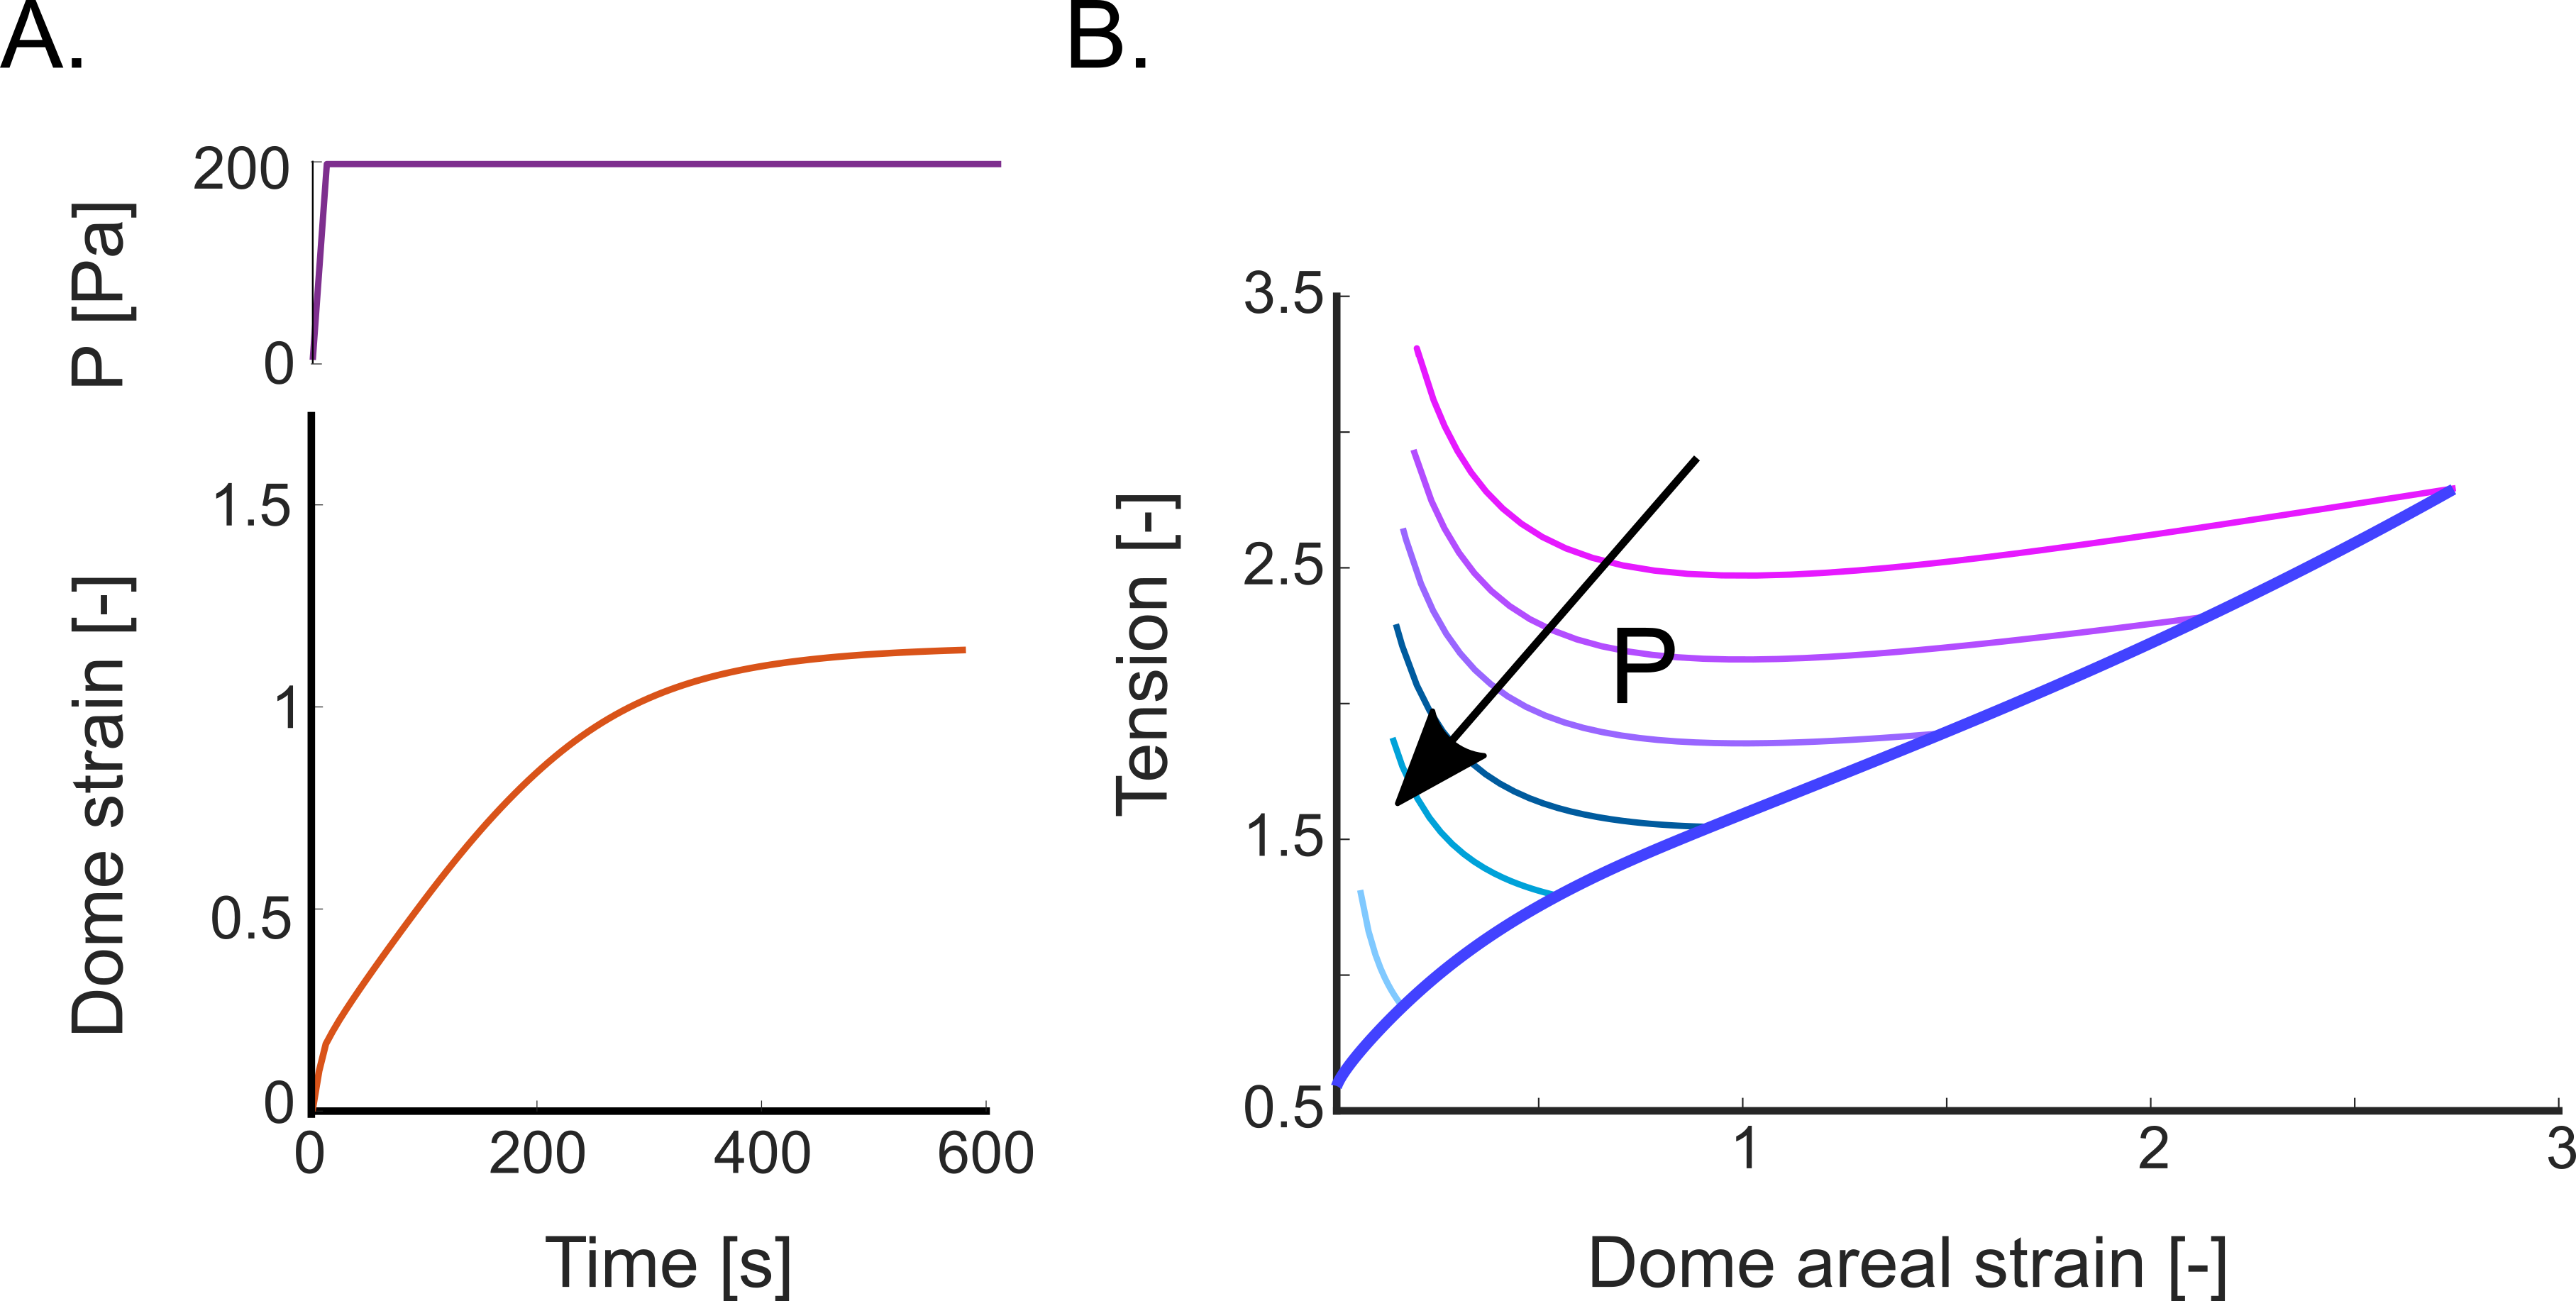
\includegraphics[width=\textwidth]{chap7_constitutivelawtwin.png}
	\caption{\label{fig_7_7} \textbf{Material response of the digital domes}: (A)  When subjected to constant pressure, as in experiments, the digital dome inflated and reached a steady state. (B)  These simulations also produced isobarics for different pressures, all leading to a steady state. Furthermore, subjecting it to a quasi-static increase in pressure produced a constitutive law (Navy blue curve) that can be mapped onto the locus of steady-state points.}
\end{figure}

\begin{figure}
	\centering
	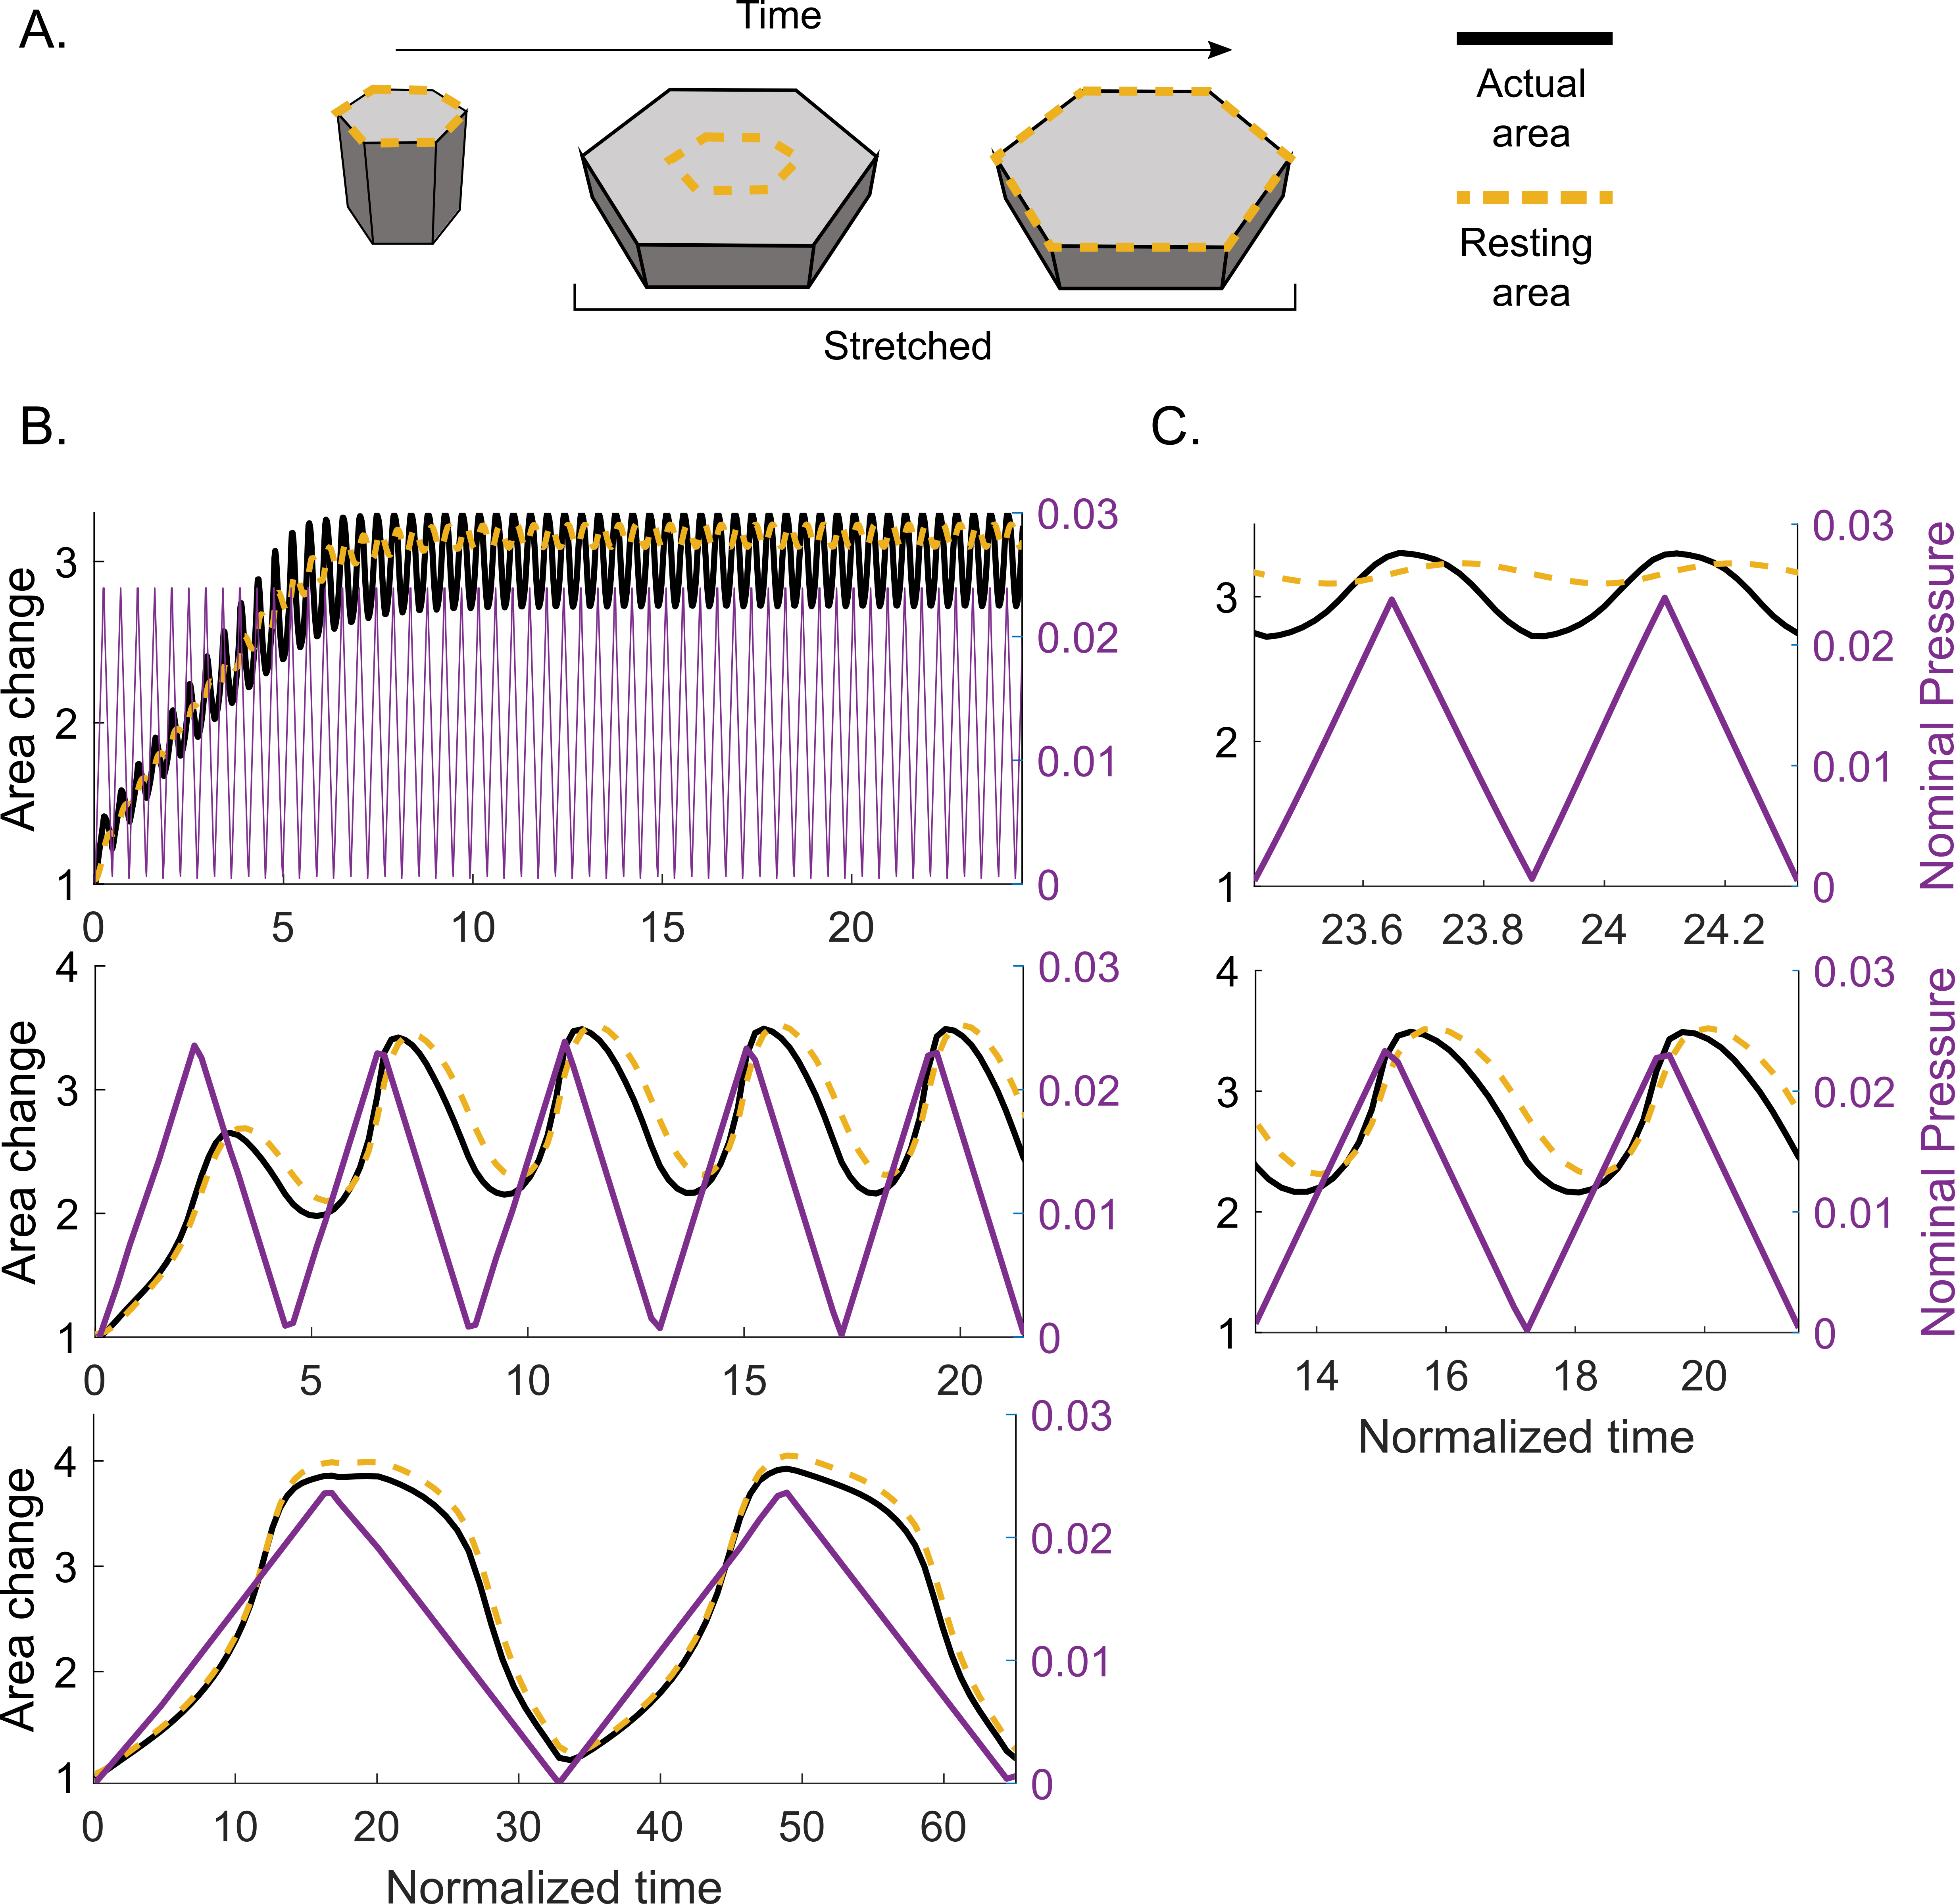
\includegraphics[width=\textwidth]{chap7_area.png}
	\caption{\label{fig_7_8} \textbf{Concept of resting area}: (A) Illustration of a resting and actual are of a cell in a monolayer during stretching. (B) Differences in results of resting and actual area when subjected to different rates of pressure. (C) Inset of the last two cycles.
	}
\end{figure}

\newpage
\hypertarget{summary}{%
	\section{Summary and Discussion}\label{summary}}

In this chapter, we investigated the mechanics of epithelial tissue by applying pressure at varying rates. Initially, we applied a constant pressure of 200Pa, which led to the dynamic inflation of domes and eventually reached a steady-state in strain. Due to the spherical geometry of the tissue, we observed a non-monotonous tension-strain curve in response to the constant pressure. However, we found that the true tension-strain curve exhibited increasing tension with respect to strains at lower values, but at higher strains, the tension appeared to be independent of the strains.

Furthermore, our measurements showed that the domes accumulated strain through the cycles when probed with fast-changing pressure and reached a steady-state in later cycles. However, when stretched slowly, the domes stretched to higher strains without accumulating strain at the end of the cycle.

To understand the behavior of epithelial tissue, we developed computational framework, which show that the response of the domes to cyclic pressure is dependent on active viscoelasticity.

The tissue stretches to balance the tissue tension with externally applied pressure timescale and reaches a steady-state strain by actively remodeling the cortex. Our digital dome studies indicated that different timescales play a role together in producing the tissue’s response to pressure. These timescales are the reflection of interplay between cortical turnover, crosslinkers, and network reorganization which allows for large deformations and rapid shape changes.

Our results can be interpreted using a multidimensional Maxwell model, which is a model that describes viscoelasticity. The classical Maxwell model consists of a spring and a dashpot, which represent the elastic and viscous elements, respectively. In our case, we can imagine a similar model with two branches: one branch includes a spring and a dashpot to represent the passive viscoelasticity, and a second branch includes an active spring to represent the active component  (see fig \ref{fig_7_9}). The active spring is always present, but if the system is stretched slowly, the dashpot would be driving the dominant mechanical response. Conversely, if stretched rapidly, the elastic spring deformation would dominate. By separating the passive and active components, we can better understand how each contributes to the overall viscoelastic behavior and associated timescales.

Previous research has approached the system in a similar manner, where epithelial tissue was modeled using viscoelastic models of springs and dashpots. One particularly interesting model was developed by Khalilgharibi et. al., which characterizes the response of a suspended monolayer to stretch and demonstrates that the dynamics are similar to that of a single cell, due to the role of the actomyosin cortex \cite{khalilgharibi2019}. They used a model with two springs in parallel, one of which can change its resting length dynamically. This explains the relaxation of the monolayer, where the active contractility of the cortex changes the resting length of the active spring in the model, which closely relates to our "resting area" concept.

Another study found that viscoelastic dissipation could explain the shortening or elongation of cell junctions in drosophila embryos \cite{clement2017}. They demonstrated that the dissipation occurs at the minute timescale, at the same timescale as myosin pulses. It is also interesting that they found actin turnover plays a key role in this dissipation.

Applying tensions and strains to suspended cells in vitro is a challenging task, and it is important to note that adherent monolayers may exhibit different behaviors from suspended cells \cite{harris2012}. The tissue matrix provides additional stiffness and can alter the cytoskeletal structure of cells, which further complicates the understanding of cell mechanics \cite{humphrey2014, kechagia2019}. In this thesis, we focused on probing the response of suspended tissues at the short timescales (minutes), which is the timescale of acto-myosin network remodeling.

We did not observe any cellular rearrangement, extrusion, or division at this timescale in our system (with rare exceptions). Long-term experiments were not performed due to suspected involvement of other cytoskeletal components, such as intermediate filaments. In a study by Latorre et al., activation of intermediate filaments was observed in extremely stretched cells (>300\%), where they proposed that this is caused re-stiffening and prevented the cells from stretching too much  \cite{latorre2018}. This motivated the strain limiting mechanism imposed in our model. However, in our experiments, we did not observe any indication of superelasticity, as all cells were super-stretched at the same time. This might be due to the relatively shorter timescales in our experiments compared to long term quasi-static deformation of spontaneous domes.

\textbf{About strain stiffning and results of \cite{duque2023}. About racheting of contractile force \cite{clement2017, mason2011} and strain accumulation or creep}

In the next chapter, we will endeavor to apply our understanding of viscoelasticity to generate radical transformation of domes into various structures.

\begin{figure}
	\centering
	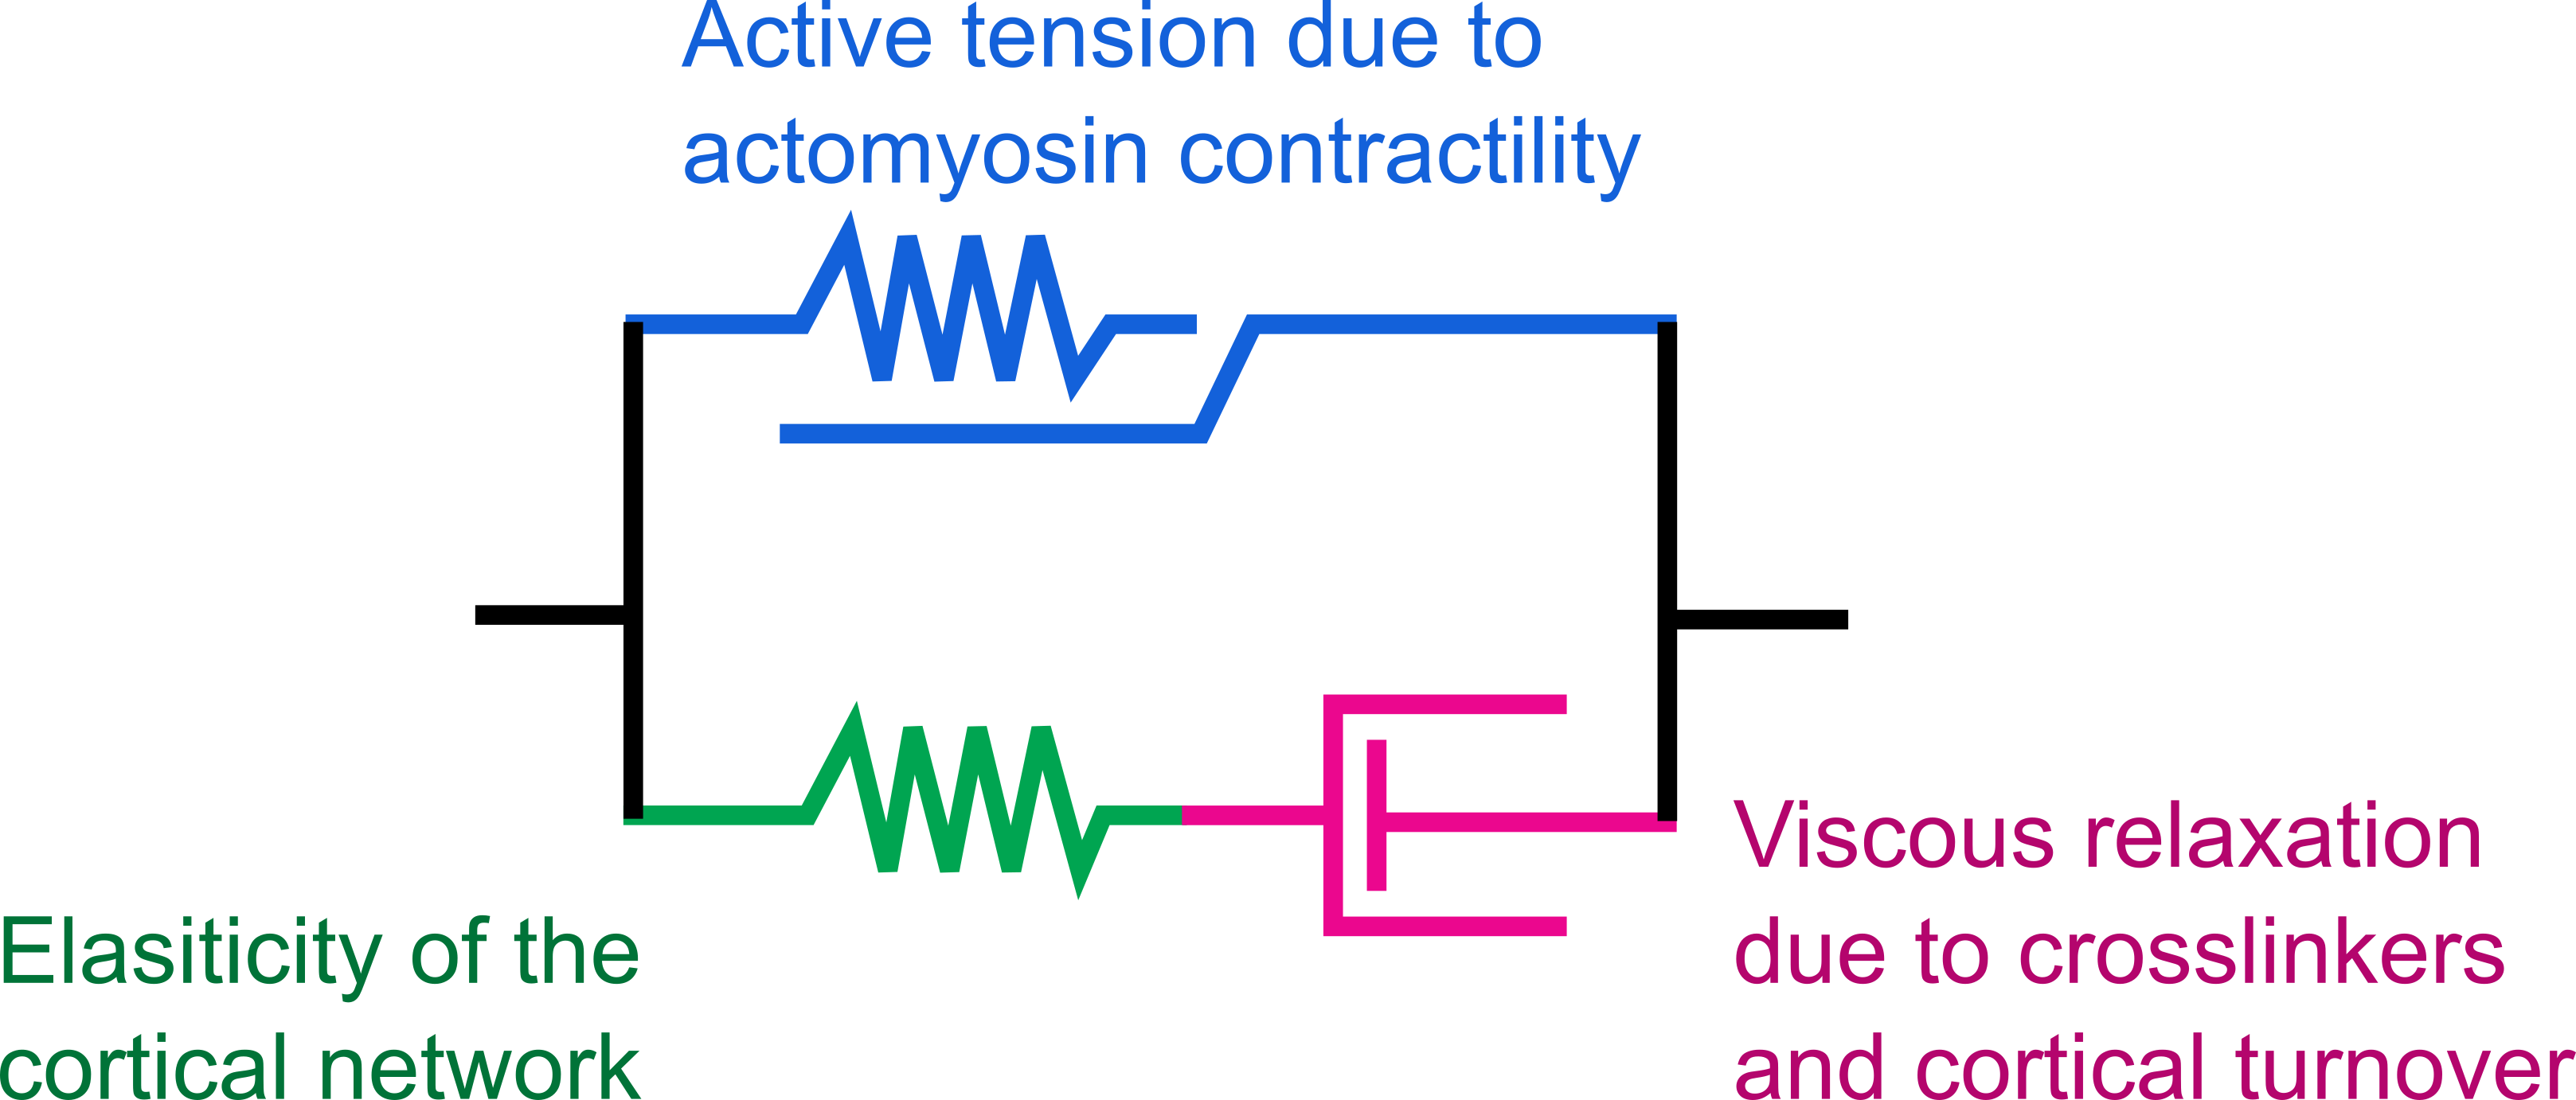
\includegraphics[width=0.75\textwidth]{chap7_maxwell.png}
	\caption{\label{fig_7_9} \textbf{Representational viscoelasticity model}: The model can be understood using a spring and dashpot analogy with two branches: The first branch is an active spring representing the contractile forces applied by the actomyosin cortex. The second branch has two components, one for the elasticity of the network and the second for the viscous relaxation that occurs due to turnover of the network.
	}
\end{figure}